\chapter{Background Modeling}\label{bkg_estimate}

To perform an accurate prediction of the SM backgrounds we used a data-driven strategy called \emph{alpha ratio method} that will be discuss in the section \ref{alpha}. The dominant background contribution in the analysis  originates from the V+jets processes (they represent the 83$\%$ of the total background). The subdominant contributions come from $t\bar{t}$, diboson (WW/WZ/ZZ), and QCD multijets. The subdominant contribution yields and the transverse mass shapes ($M_{VZ}^{T}$) are primarily taken from simulation. Table \ref{tab:backgrounds} summarize the background categories.

\begin{table}[!ht]
\begin{center}
\caption{Background categories.}
\label{tab:backgrounds}
\begin{tabular}{lc} \hline
Category & Backgrounds \\ \hline
Dominants &  $W$+jets($W \rightarrow \ell \nu$), $Z$+jets ($Z\rightarrow \nu \nu$)  \\
Subdominants   &  Multijets, $t\bar{t}$, dibosons ($WW$/$WZ$/$ZZ$) \\ \hline
\end{tabular}
\end{center}
\end{table}

To determine the dominant V+jets background in the signal region ($m_{\text{jet}} \in \left[65,105 \right]$ GeV), a signal-free sideband region is defined in the mass of the hadronic V candidate by the interval  $m_{\text{jet}} \in \left[40,65 \right] \cup \left[135,220\right]$ GeV. The region $m_{\text{jet}} \in \left[105,135 \right]$ GeV is not used in order to avoid any bias in the $M_{VZ}^{T}$ shape due to possible contributions from new resonances in the HZ final state, in which the Higgs bosons would decay to a pair of b-quarks. Table \ref{tab:jetmassregions} summarize the different jet mass regions used for the background modeling.

\begin{table}[!ht]
\begin{center}
\caption{Jet mass regions.}
\label{tab:jetmassregions}
\begin{tabular}{lc} \hline
Region & Interval (GeV) \\ \hline
Lower sideband  (LSB) &  $\left[40,65 \right]$  \\
Lower signal  (SR)  &  $\left[65,105 \right]$ \\ 
Upper signal (Higgs) & $\left[105,135 \right]$   \\
Upper sideband (USB) & $\left[135,220 \right]$  \\ \hline
\end{tabular}
\end{center}
\end{table}

In general, we experience low statistics in data, particularly in the tail of transverse mass distribution, which is the main observable in order to determine any possible signal of new physics. For those cases unbinned maximum likelihood (ML) fits are preferred due to robustness (statistically more powerful) and to avoid the information loss and arbitrariness of the binning procedure \cite{Verkerke:2003ir}. Therefore, in the analysis, we perform all the fits using the unbinned ML method.

\section{Alpha ratio method}\label{alpha}

The alpha ratio method is based on the extrapolation of the background shape and yield from the jet pruned mass sideband to the signal region. The method relies on the assumption that the correlation between $M_{VZ}^{T}$ and the  jet pruned mass for the dominant background in data is reasonably well reproduced in simulation. The advantage of this approach is that most systematic uncertainties cancel in the ratio.
The total background prediction (normalisation and shape) as a function of the reconstructed resonance mass, $M_{VZ}^{T}$, is obtained separately for each purity category according to the formula:

\begin{eqnarray}
N_{\text{total}}^{\text{signal}}(M_{VZ}^{T}) &=& N_{\text{DB}}^{\text{signal}}(M_{VZ}^{T}) + N_{\text{SB}}^{\text{signal}}(M_{VZ}^{T})\\
                                        &=& \underbrace{N_{\text{data}}^{\text{sideband}}(M_{VZ}^{T}) \times (1-R_{0}(M_{VZ}^{T}))\times \alpha^{MC}(M_{VZ}^{T})}_{\text{Shape}}\times \underbrace{F_{DB}}_{\text{Norm}} \nonumber  \\                                        &+& N_{\text{SB}}^{\text{signal}}(M_{VZ}^{T})  \nonumber
\end{eqnarray}

where

\begin{itemize}
\item
$N_{\text{total}}^{\text{signal}}(M_{VZ}^{T})$ is the total background prediction in the signal region;
\item
$N_{\text{DB}}^{\text{signal}}(M_{VZ}^{T})$ is the dominant background prediction in the signal region (W/Z + jets);
\item
$N_{\text{SB}}^{\text{signal}}(M_{VZ}^{T})$ is the background prediction in signal region for the sum of the subdominant backgrounds ($t\bar{t}$, multijets, dibosons);
\item
$N_{\text{data}}^{\text{sideband}}(M_{VZ}^{T})$ is the $M_{VZ}^{T}$ distribution in data for the sideband region;
\item
$R_{0}(M_{VZ}^{T})= N_{\text{SB}}^{\text{sideband}}(M_{VZ}^{T})/N_{\text{data}}^{\text{sideband}}(M_{VZ}^{T})$ is the fraction of subdominant backgrounds in the sideband region with respect to the total background in the sideband region (i.e. data). The $1-R_{0}(M_{VZ}^{T})$ multiplicative term represents the substraction of the subdominant contribution from the data in the sideband region;
\item
$\alpha^{MC}(M_{VZ}^{T})= N_{\text{DB}}^{\text{signal}}(M_{VZ}^{T})/N_{\text{DB}}^{\text{sideband}}(M_{VZ}^{T}) $ is the dominant background prediction in the signal region divided by the one in the sideband region, calculated from MC. It represents the transfer function (from sideband to signal region) used to correct the data in the sideband region and extract the dominant background’s $M_{VZ}^{T}$ shape.
\item
$F_{DB}$ is an overall scale factor used to set the normalisation of the dominant background prediction.
\end{itemize}

In summary, the method is divide in two parts, the shape and the normalization prediction for the dominant backgrounds. We will detail each in the following sections. The alpha ratio method is the standard strategy for background estimation used by CMS in similar searches \cite{CMS:2013xea,CMS-PAS-EXO-12-022, CMS-PAS-EXO-15-002}. 


\subsection{Background normalization}

The $m_{\text{jet}}$ distribution is modeled with analytic functions on simulation, considering separately the dominant and subdominant backgrounds. The overall dominant background normalization in the signal region is determined from a fit to the $m_{\text{jet}}$  distribution in the sideband region, after fixing both the shape and the normalization of the subdominant backgrounds. Table \ref{tab:functions} show the functional forms employed to describe the jet pruned mass distribution.

\def\arraystretch{2.0}
\begin{table}[!ht]
\begin{center}
\caption{Analytic functions to fit the jet pruned mass distribution.}
\label{tab:functions}
\begin{tabular}{lcc} \hline
Name & Description & Function \\ \hline
\textbf{ErfExp} & An exponential times an error function & $e^{a} \cdot \frac{1 + \text{Erf}\left((x-b)/w \right)}{2}$ \\
\textbf{Gaus2}  &  The addition of two gaussians & $f_{0}e^{-(x-a)^{2}/2s^{2}} + (1-f_{0})e^{-(x-b)^{2}/2s^{2}}$ \\ \hline
\end{tabular}
\end{center}
\end{table}

To verify that the W + jets and Z +jets samples have the same shape and that we can treat them together as a dominant background, we perform a cross-check, fitting them separately as is shown in Figure \ref{fig:Vjets}. For the normalization procedure we follow the next steps:

\begin{itemize}
\item
We fit the dominant backgrounds with the \textbf{ErfExp} model in the total jet pruned mass distribution, as it can be observed in the top-left side of the figures \ref{fig:fitprunedHP}, \ref{fig:fitprunedLP}.
\item
We fit the subdominant backgrounds with the \textbf{Gaus2} model in the total jet pruned mass distribution, as it can be observed in the top-right side of the figures \ref{fig:fitprunedHP}, \ref{fig:fitprunedLP}.
\item
We use an extended model adding the PDFs of the dominant and subdominants backgrounds. For the dominant backgrounds we let both the parameters of the normalization and shape float and for the subdominant backgrounds we fix the parameters of the normalization and shape. Then we fit the extended model to the data in sidebands.
\item
Using the results of the fits, we predict the shape and the normalization ($F_{DB}$) of the dominant backgrounds in signal region. Figures \ref{fig:fitprunedHP}, \ref{fig:fitprunedLP}, bottom side, show the prediction  in comparison with data. In addition, we can extract the estimation of the total yields in signal region as is reported in table \ref{tab:backyields4}.
\end{itemize}

The characterization of the jet pruned mass with the analytic functions was evaluated in simulation and compared against alternative functions. To consider the mis-modelling of the pruned jet mass, an uncertainty was included as a systematic error that ranges between 15-20 $\%$. The expected and observed number of events in the signal region is given in Table \ref{tab:backyields4}; the result is reported for the HP and LP categories.

\begin{table}[!ht]
\begin{center}
\caption{Expected and observed background yields in signal region.}
\label{tab:backyields4}
\begin{tabular}{lcccc} \hline
Category & Background &  Expected & Observed & Syst. Uncer.\\ \hline
HP & Dominant + Sub-dominant  &  544 $\pm$ 40  & 507 & 20.5 $\%$  \\
LP & Dominant + Sub-dominant  &  820 $\pm$ 53 & 806  &  15.5$\%$  \\ \hline
\end{tabular}
\end{center}
\end{table}

\subsection{Background shape}

Evidence of a new resonance decaying into disboson ($VZ$) would appear as a localized excess in the transverse mass distribution. Because of this, it is essential to perfom a good estimtaion of the background shape in the $M_{VZ}^{T}$ variable. Due to the correlation between the jet pruned mass and the transverse mass variables, the selections on the $m_{\text{jet}}$ reported in table \ref{tab:jetmassregions} define the sideband and the signal regions in the $M_{VZ}^{T}$ distributions. The analytic model selected to estimate the background shape of the transverse mass distribution is the \textbf{ExpTail}:
\begin{eqnarray}
F_{\text{ExpTail}}(x) = e^{-x/(a+bx)}
\end{eqnarray}
The choice of the functional forms for the VZ transverse mass for different categories is shown in table \ref{tab:trasnversefunctions}.
\begin{table}[h]
\begin{center}
\caption{Summary of the shapes used for fit the $M_{VZ}^{T}$ spectra of each category.}
\label{tab:trasnversefunctions}
\begin{tabular}{lcccc} \hline
Category & Fit Function & Regions & Sample \\ \hline
HP  &  ExpTail  &  signal and sideband  & Data and MC \\
LP  &  ExpTail  &  signal and sideband  & Data and MC \\ \hline
\end{tabular}
\end{center}
\end{table}

In order to predict the shape of the dominant backgrounds we follow the next steps:

\begin{itemize}
\item
We fit the subdominants backgrounds with an \textbf{ExpTail} model in sideband and signal region. After the fit we fix all the parameters of the model.
\item
We substract the subdominant backgrounds from data in the sideband region.
\item
We perform a simultaneous fit using the \textbf{ExpTail} model for the dominant background in the signal and sideband region and for the data in sideband region.
After the fit we fix all the parameters of the model. Figures \ref{fig:fits3}, \ref{fig:fits4} show the results of the fits. The top side shows the dominant backgrounds fits in sideband and signal region and the right-center side show the data fit in sideband region.
\item
We extract the alpha transfer function using the fits of the dominant backgrounds in sideband and signal region. $\alpha^{MC}(M_{VZ}^{T})= N_{\text{DB}}^{\text{signal}}(M_{VZ}^{T})/N_{\text{DB}}^{\text{sideband}}(M_{VZ}^{T})$.  Figures \ref{fig:fits3}, \ref{fig:fits4} show the alpha transfer function for high and low purity categories respectively.
\item
We predict the shape of the dominant backgrounds in signal region just correcting the $M_{VZ}^{T}$ distribution of the data in sideband region with the transfer function. Figures \ref{fig:fits3}, \ref{fig:fits4} show the final prediction in comparison with data. In those plots the normalization factor was already applied.
\end{itemize}

\begin{figure}[!ht]
\caption{ Top : Z/W +jets fits in the HP category. Center : Z/W +jets fits in the LP category. Bottom : Comparison between the Z +jets and W +jets fits.}
\begin{tabular}{cc}
  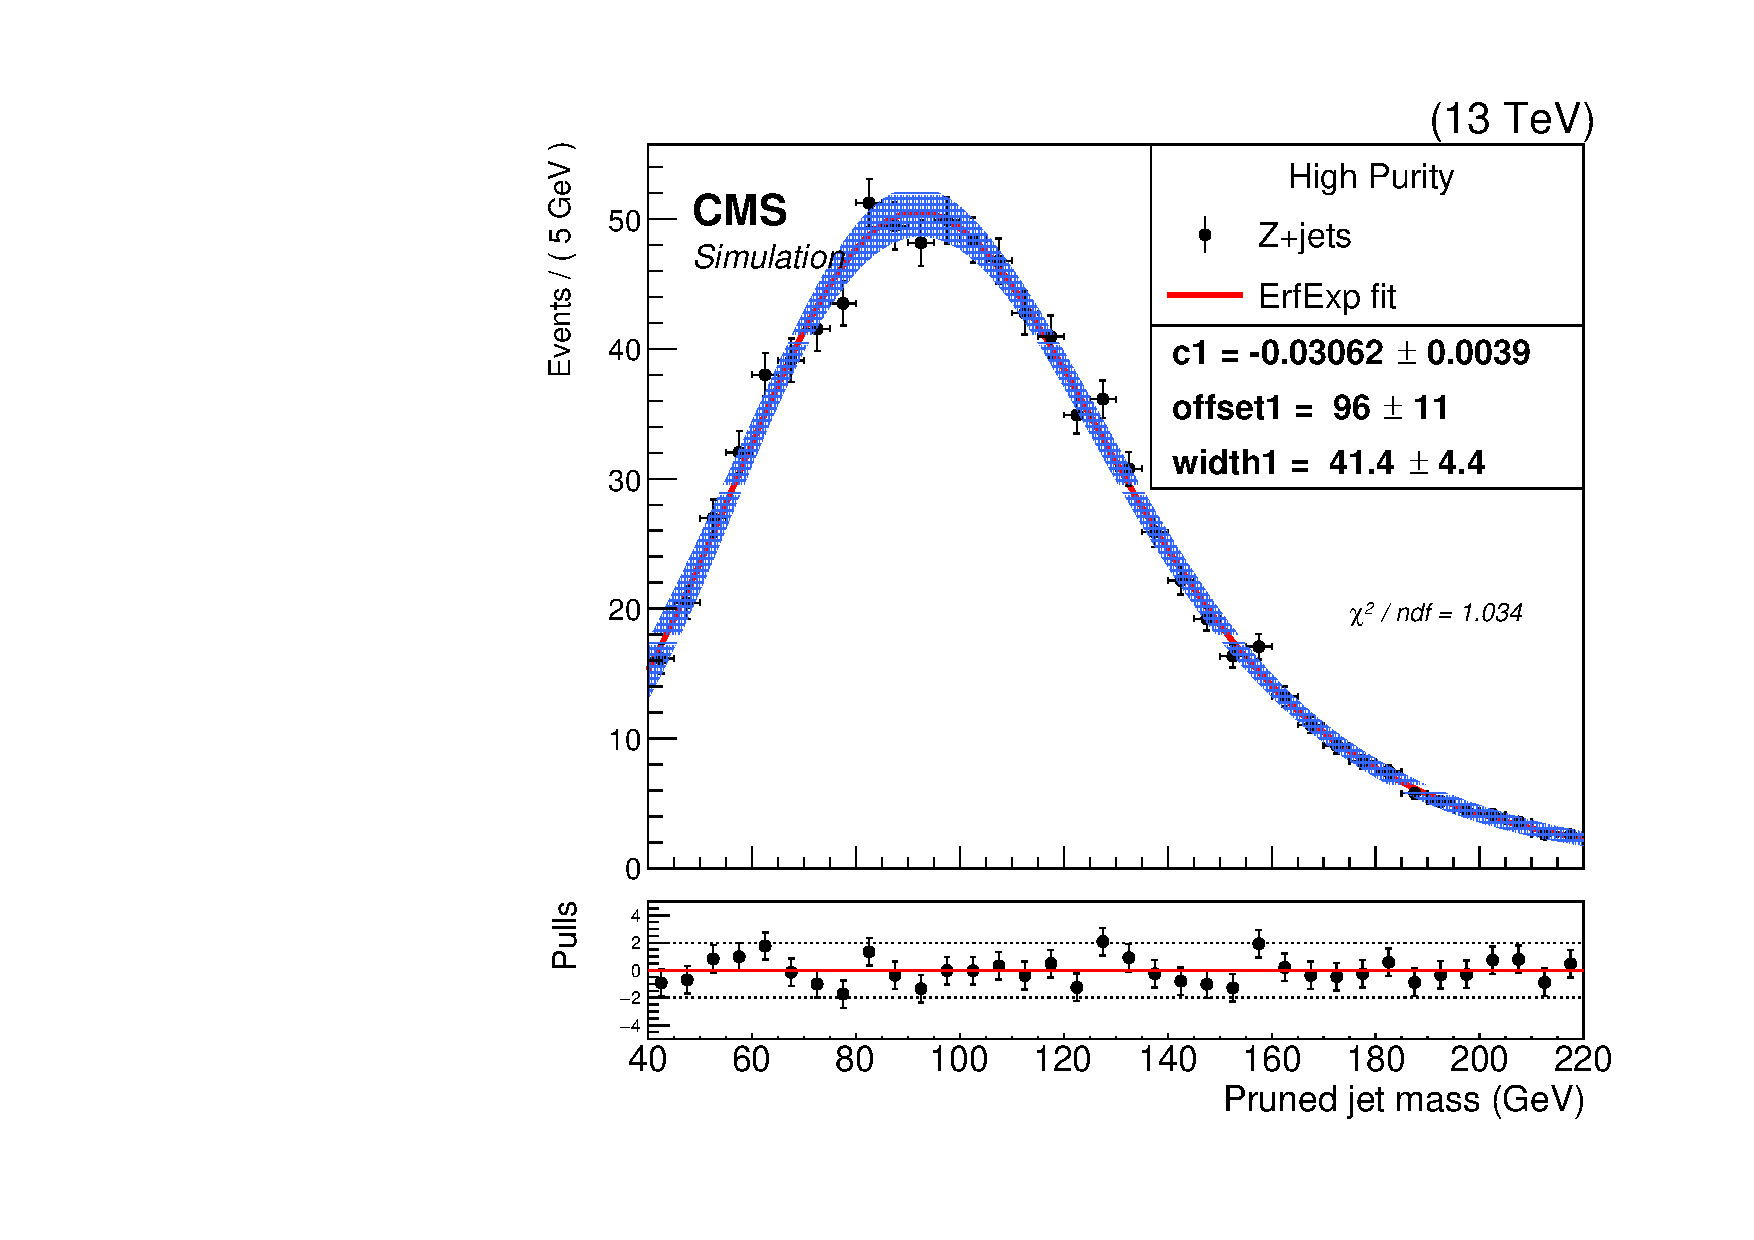
\includegraphics[width=220pt]{figuresARC/Vjets/ZjetsHP.pdf} &
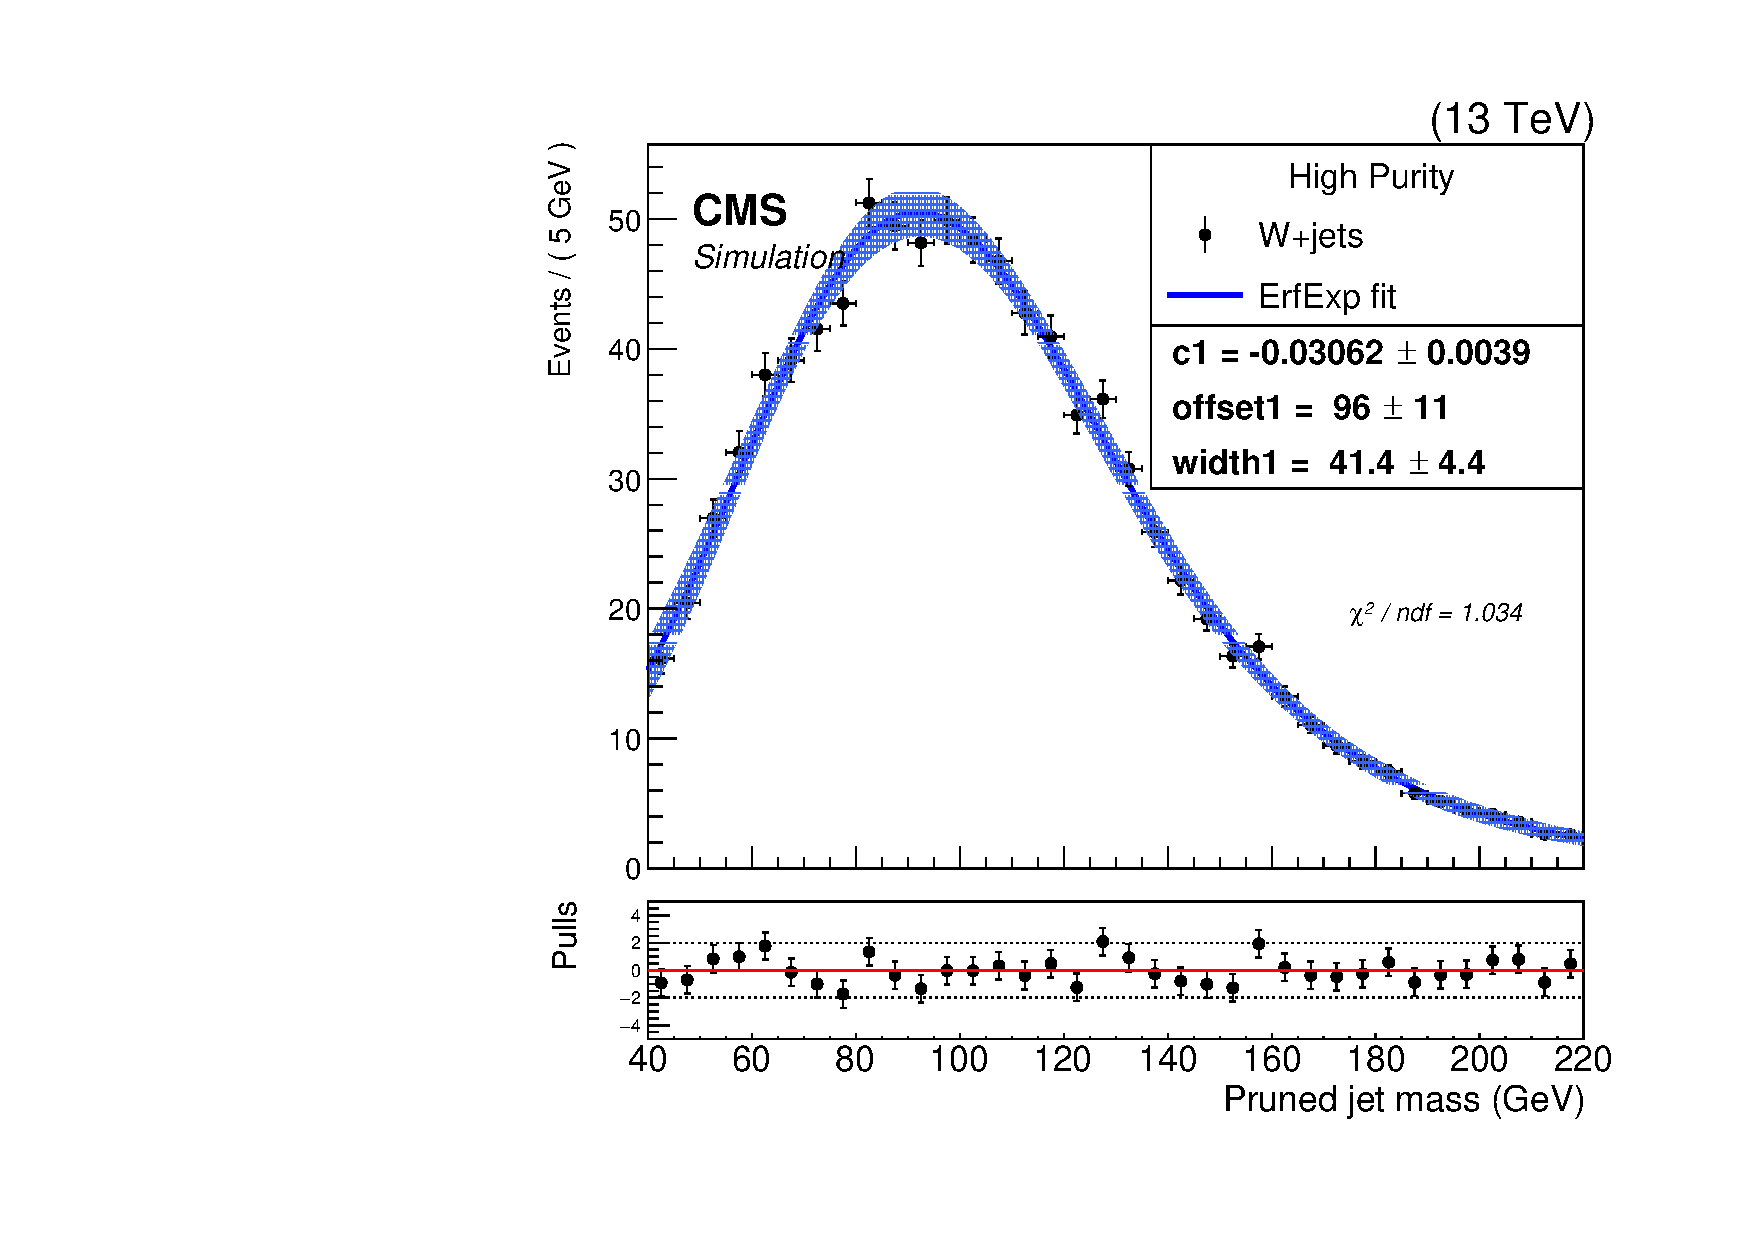
\includegraphics[width=220pt]{figuresARC/Vjets/WjetsHP.pdf}\\
  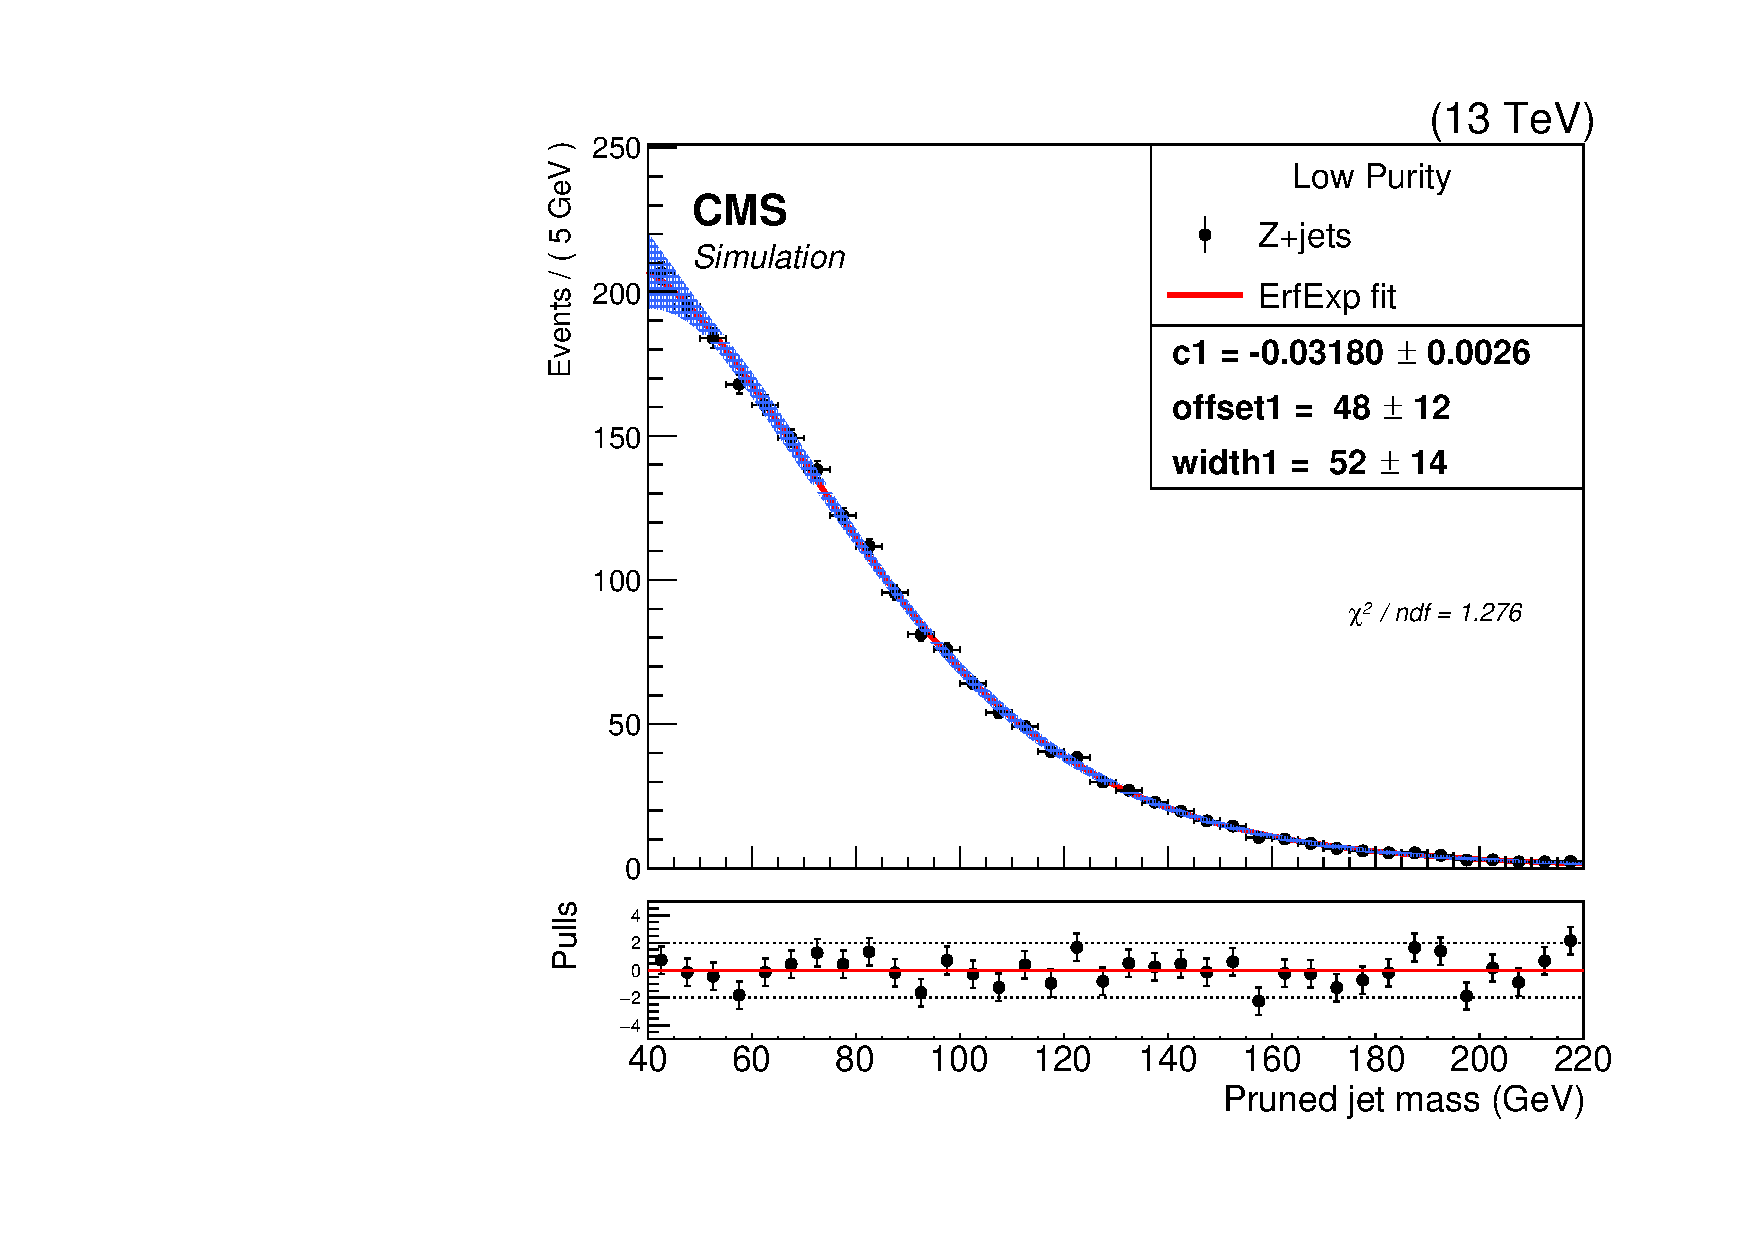
\includegraphics[width=220pt]{figuresARC/Vjets/ZjetsLP.pdf} &
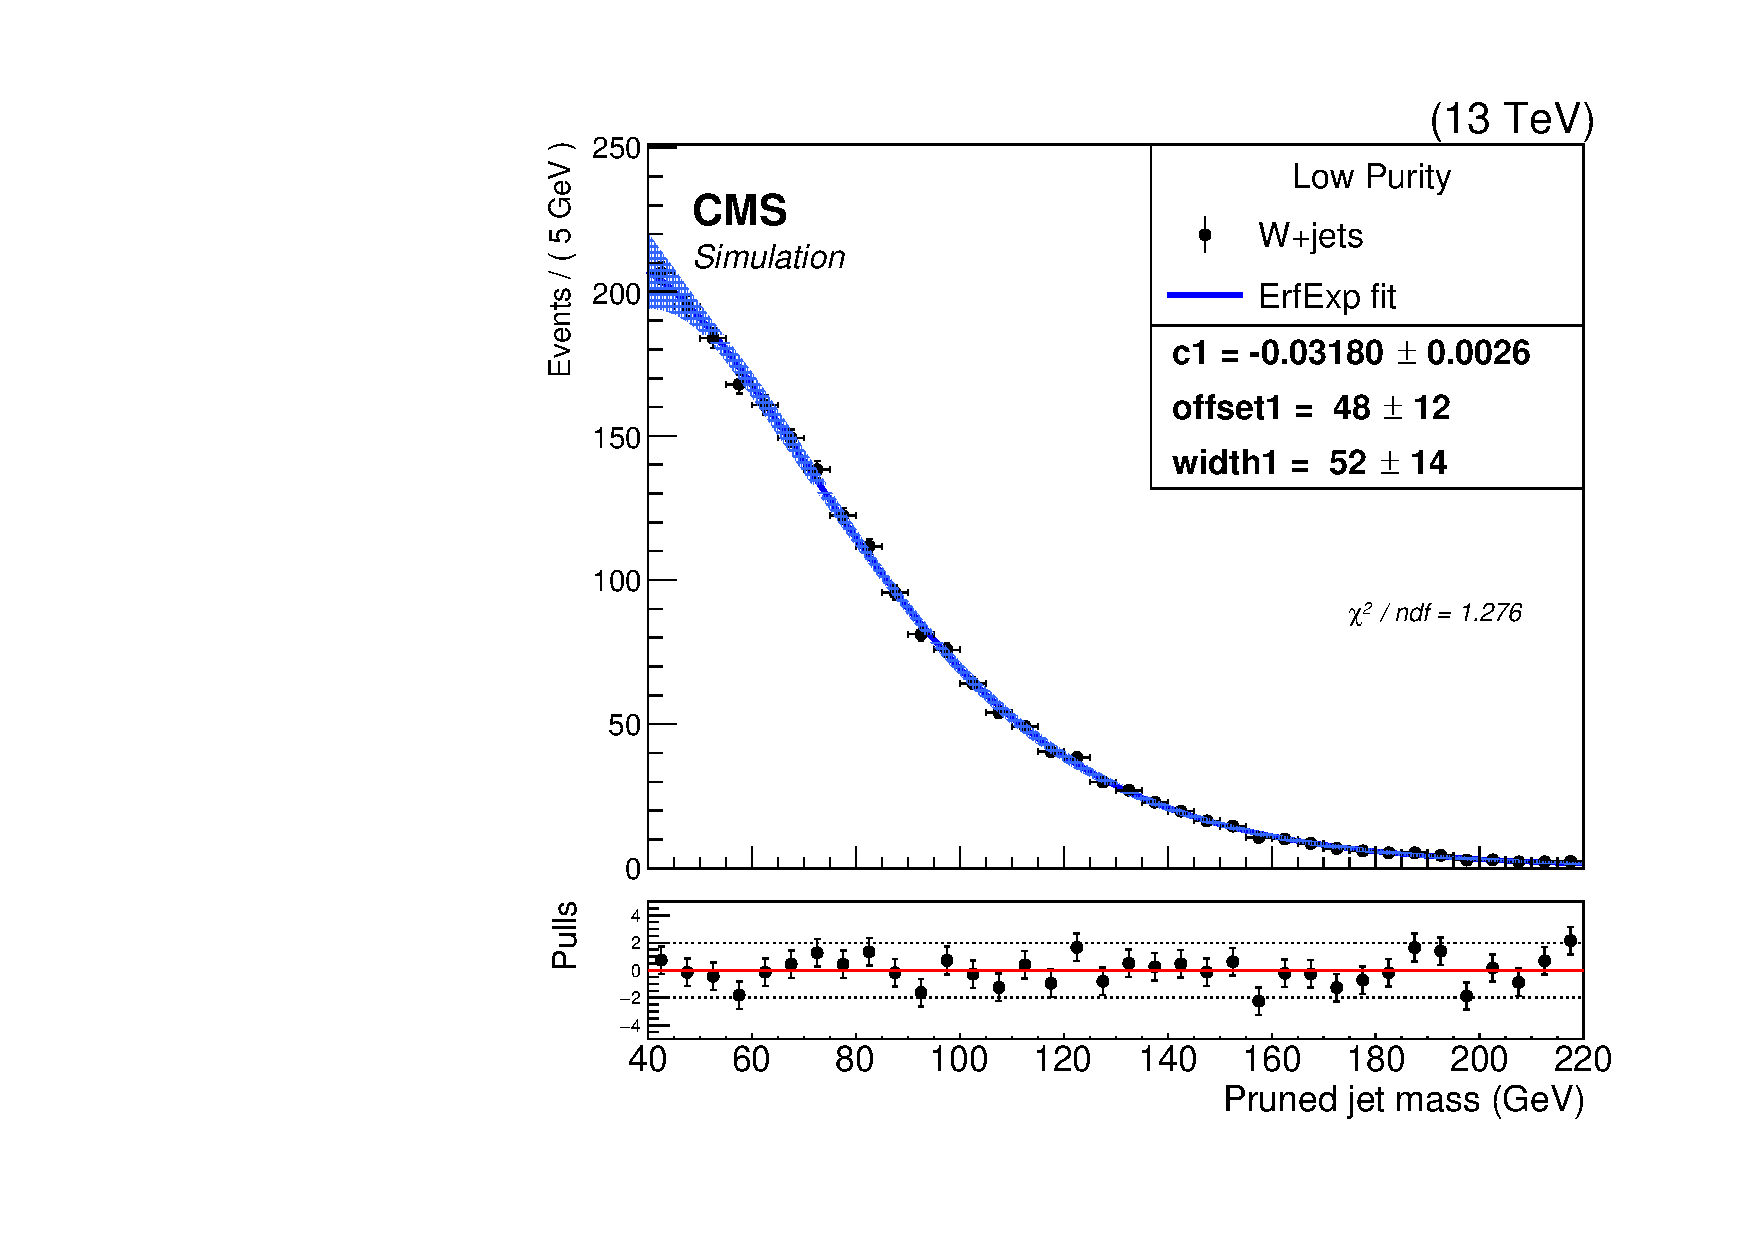
\includegraphics[width=220pt]{figuresARC/Vjets/WjetsLP.pdf}\\
  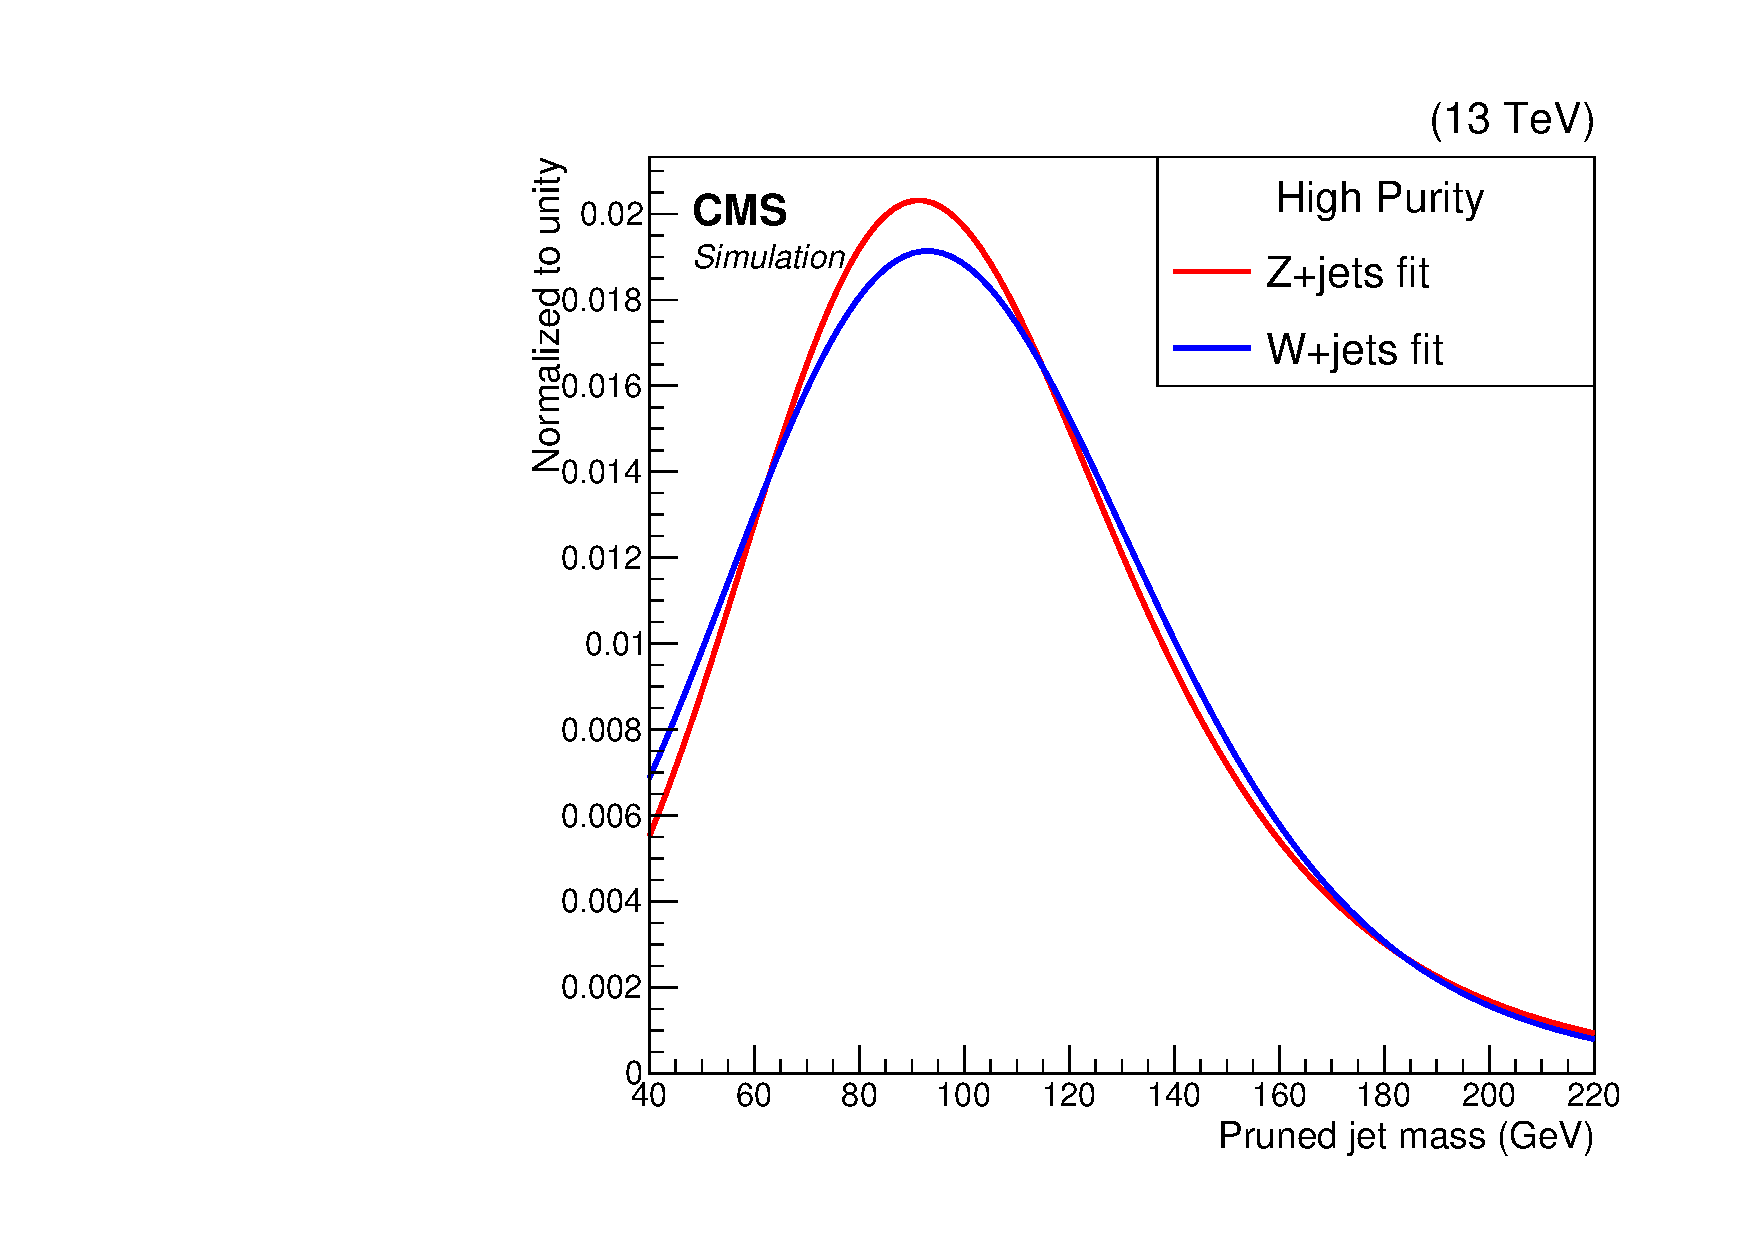
\includegraphics[width=220pt]{figuresARC/Vjets/VjetsHP.pdf} &
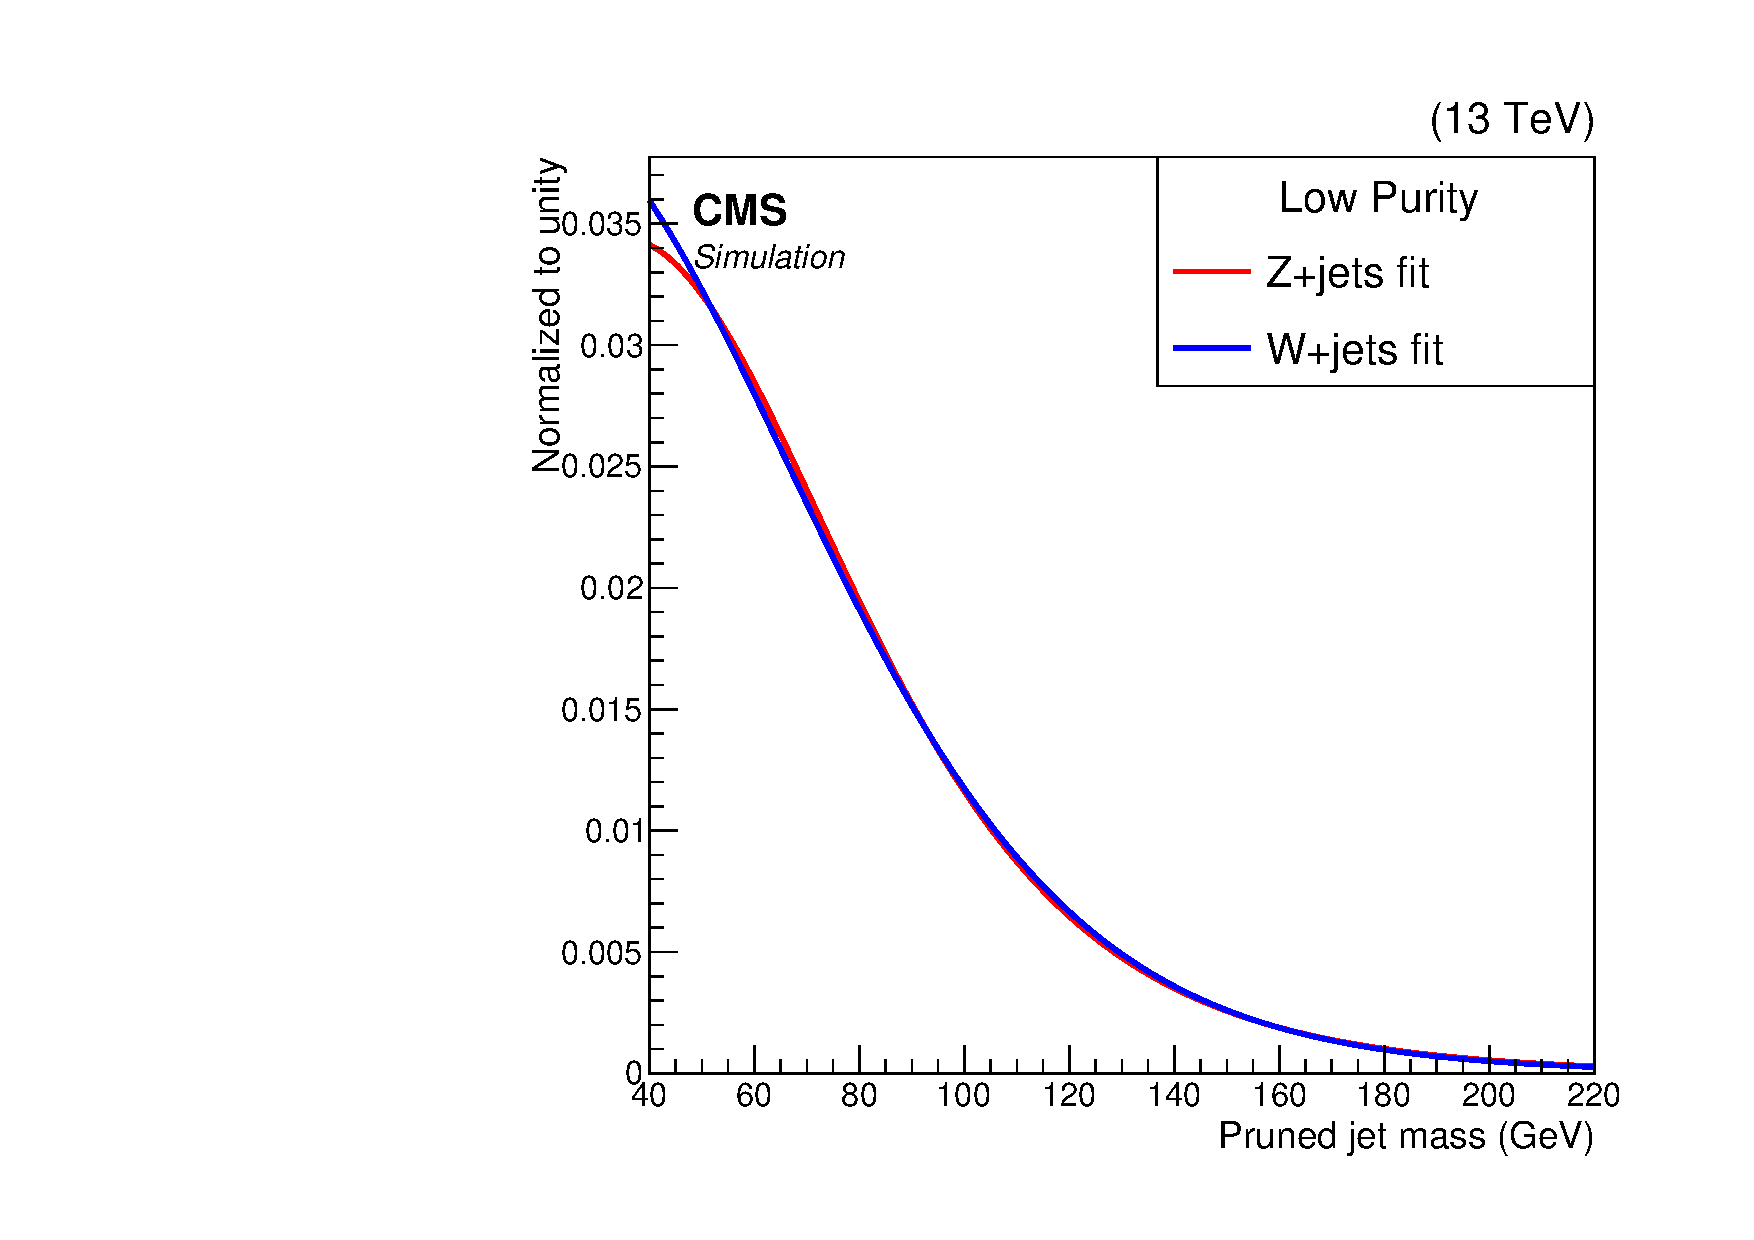
\includegraphics[width=220pt]{figuresARC/Vjets/VjetsLP.pdf}\\
\end{tabular}
\label{fig:Vjets}
\end{figure}

\begin{figure}[!ht]
\caption{ Fit of the jet pruned mass in the HP category. Top: (left) Dominant MC background fit with the ErfExp function (right) Subdominant MC background fit with the Gaus2 function. Bottom: Distribution of the jet pruned mass in the HP categories. All selections are applied except the final $m_{\text{jet}}$ signal window requirement. Data are shown as black markers. The contribution of the V+jets background is extrapolated from the sideband to the signal region.}
\begin{tabular}{cc}
  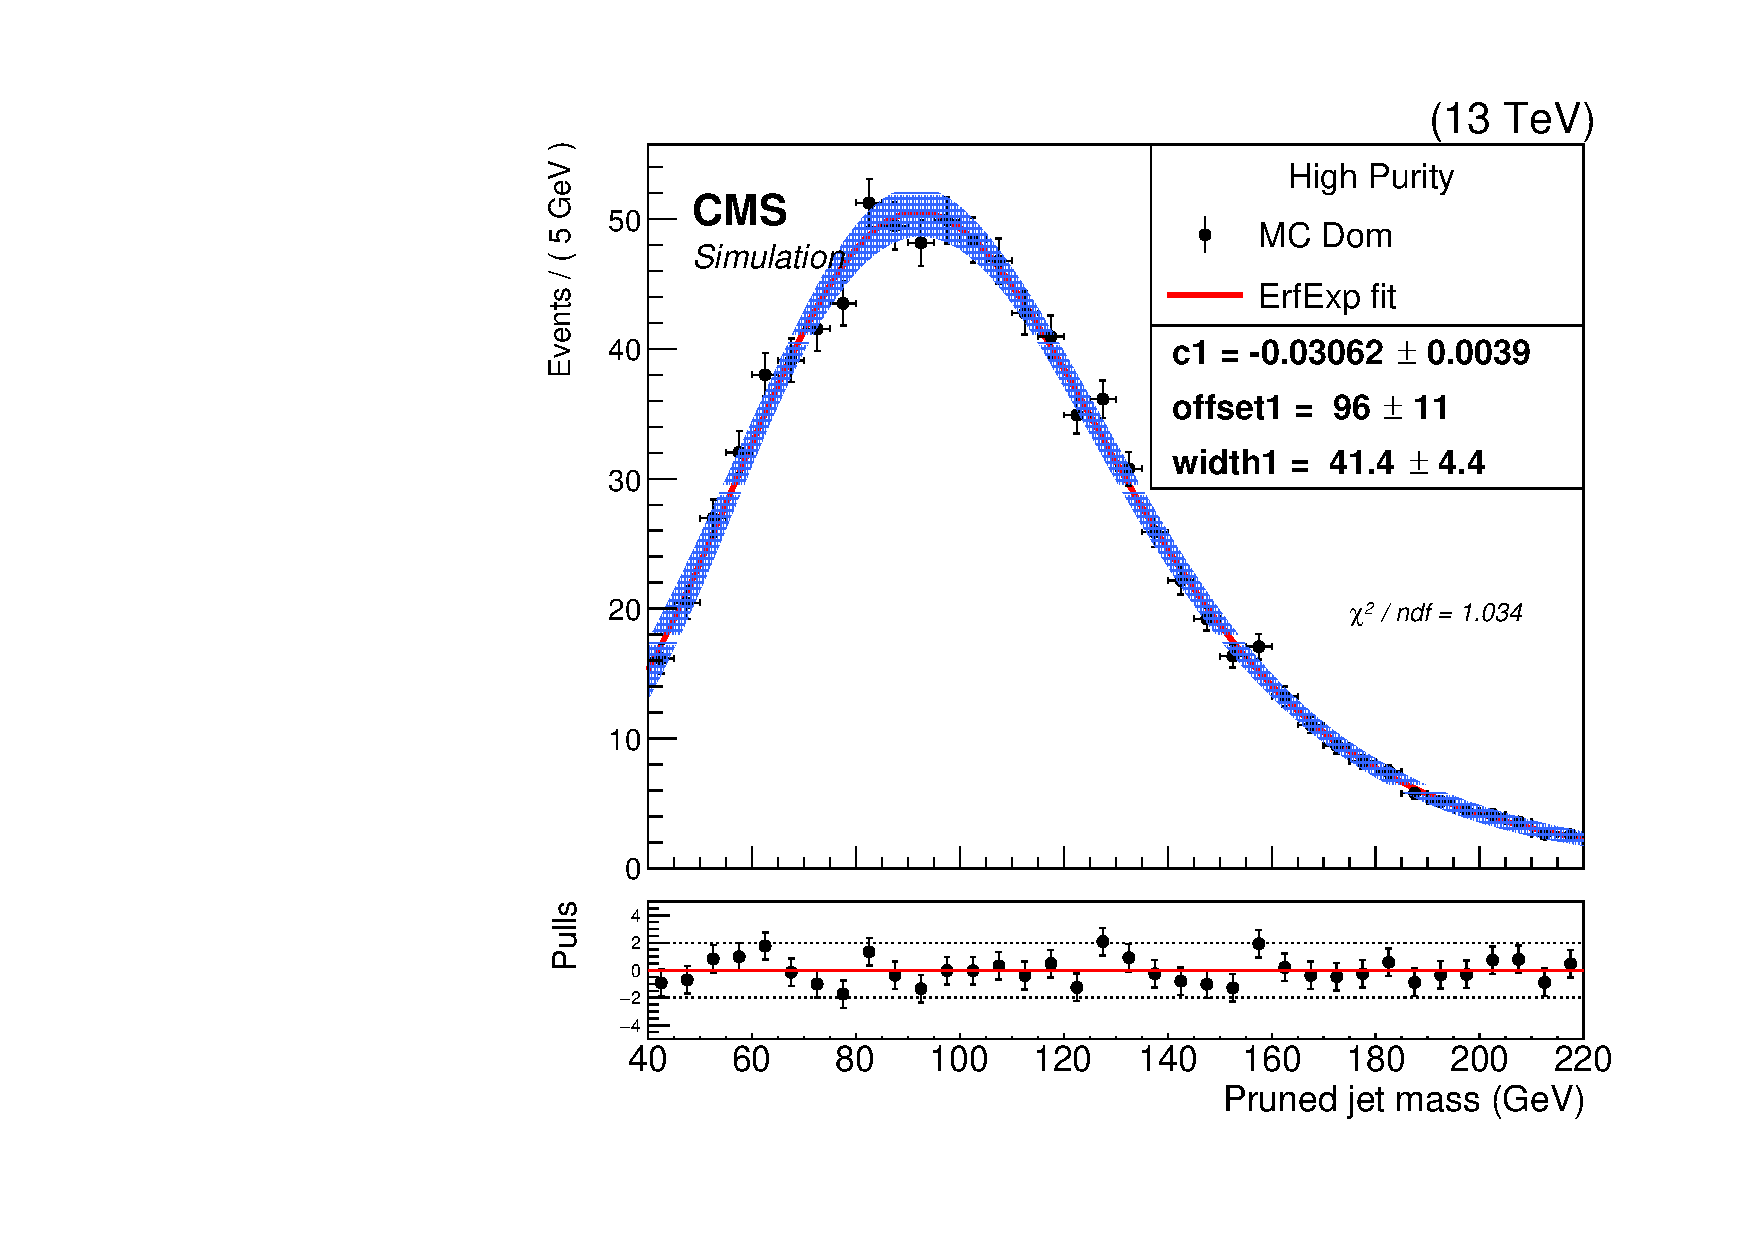
\includegraphics[width=250pt]{figuresARC/Vjets/DomHP.pdf} &
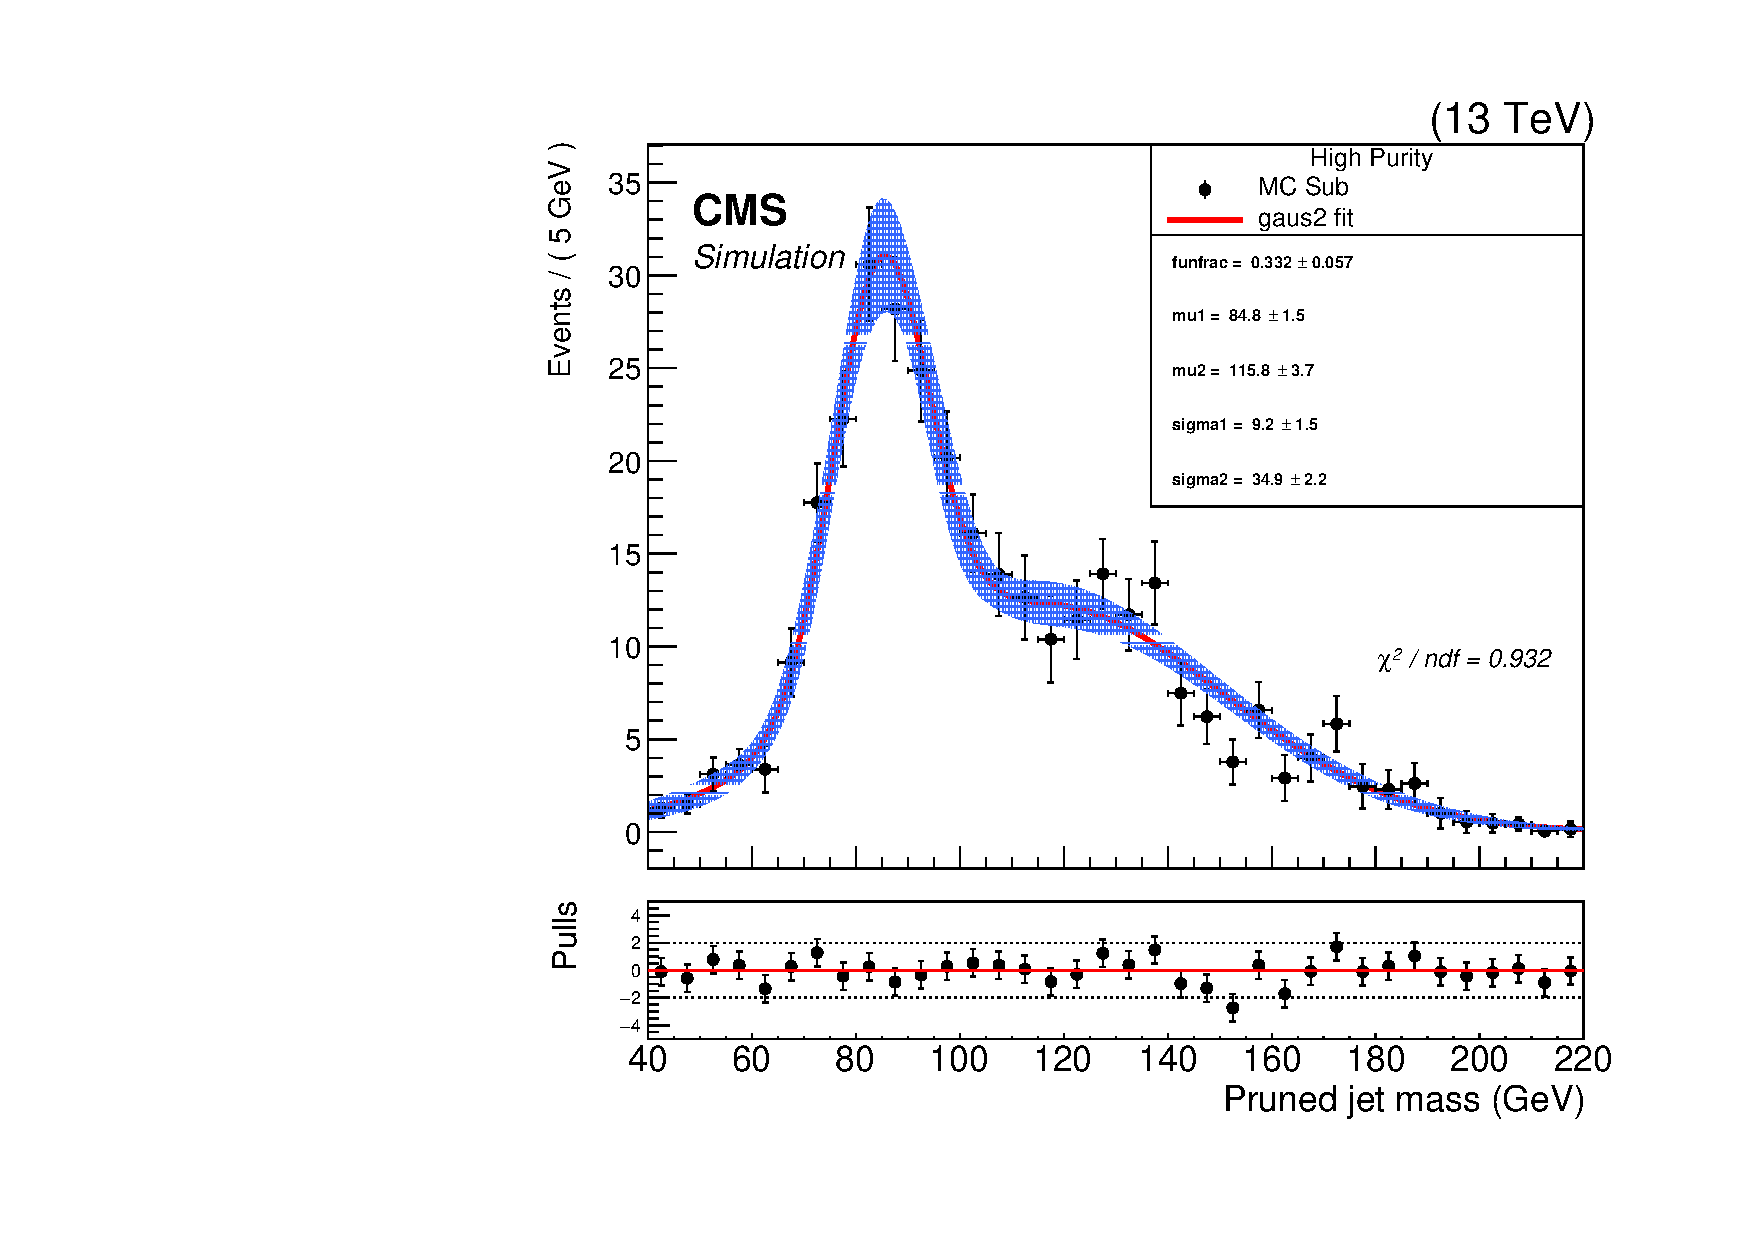
\includegraphics[width=250pt]{figuresARC/Vjets/SubDomHP.pdf}\\
\end{tabular}
\begin{center}
  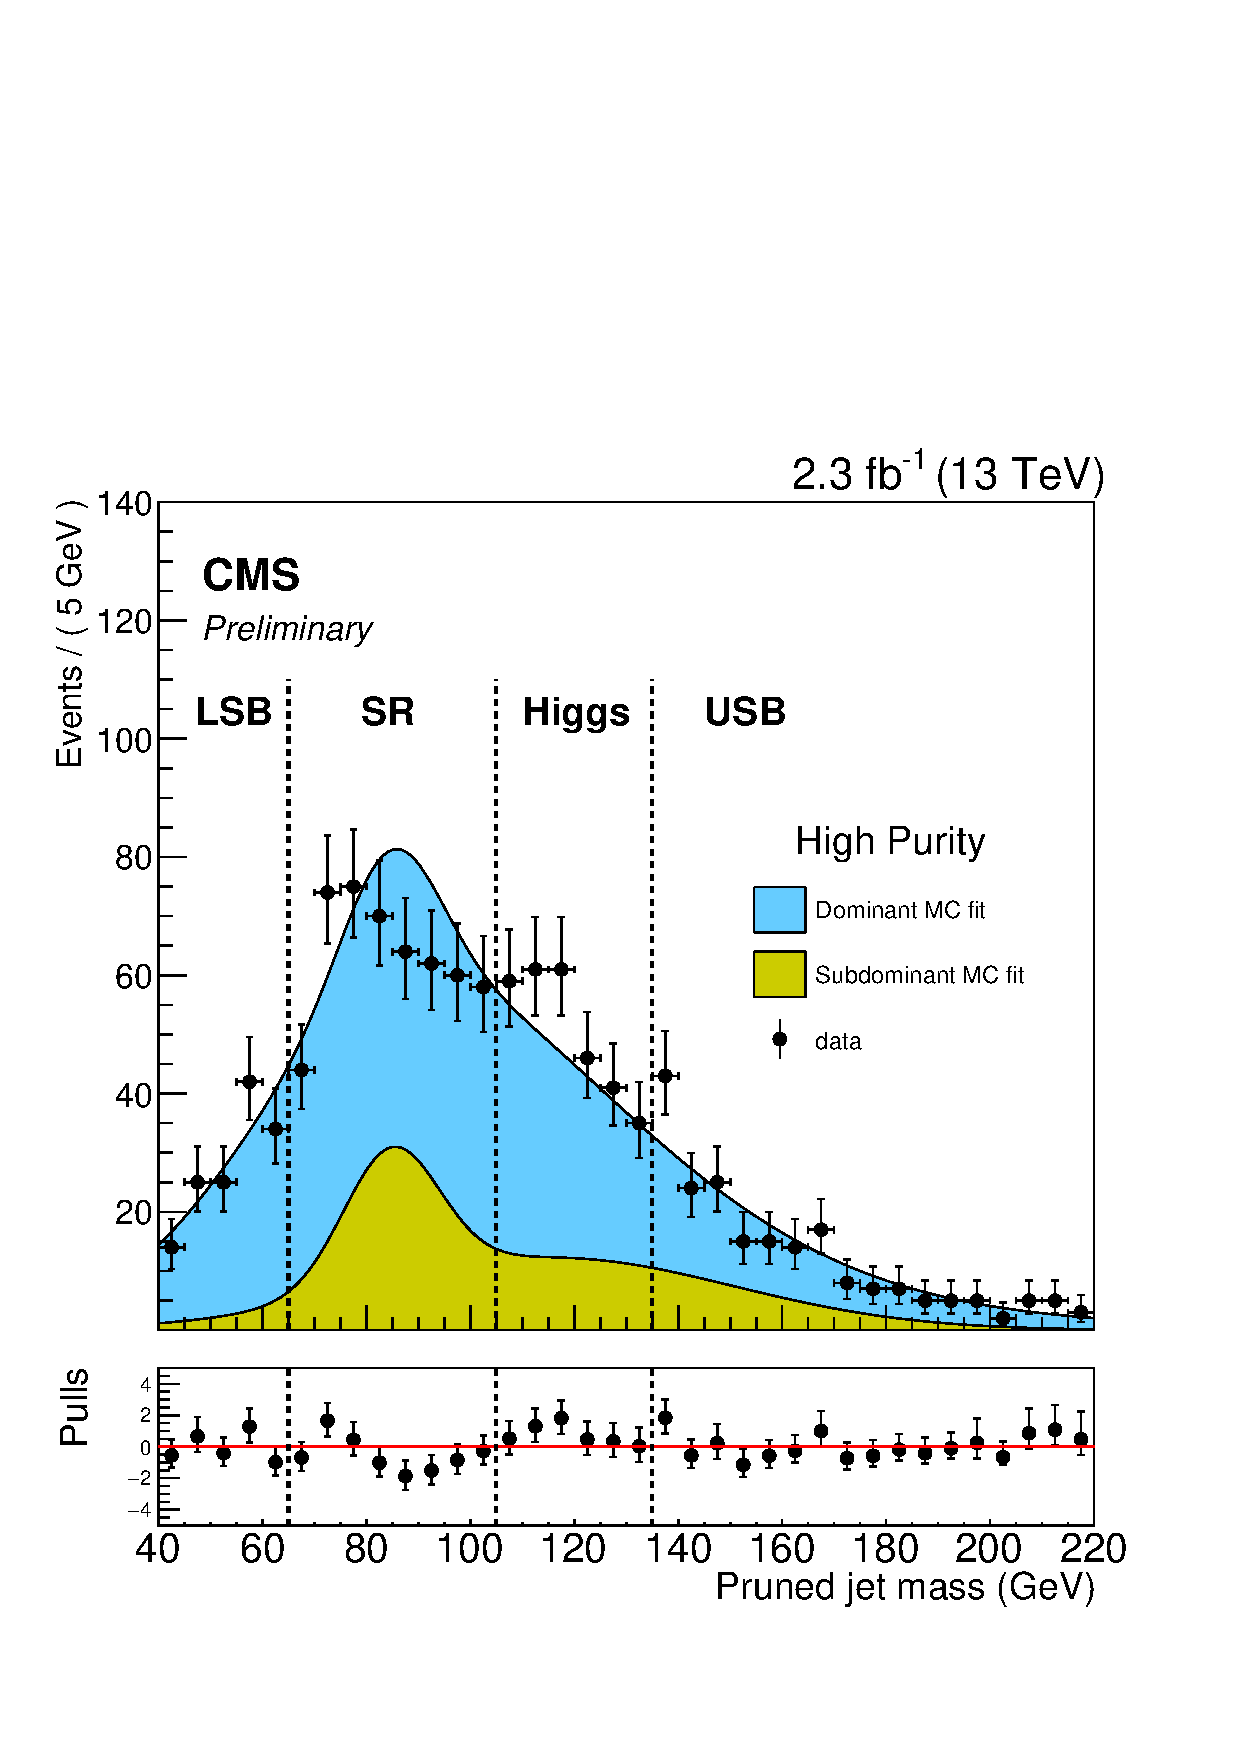
\includegraphics[width=270pt]{figuresARC/Vjets/dataMjUB3HP.pdf}
\end{center}
\label{fig:fitprunedHP}
\end{figure}

\begin{figure}[!ht]
\caption{ Fit of the jet pruned mass in the LP category. Top: (left) Dominant MC background fit with the ErfExp function (right) Subdominant MC background fit with the Gaus2 function. Bottom: Distribution of the jet pruned mass in the LP categories. All selections are applied except the final $m_{\text{jet}}$ signal window requirement. Data are shown as black markers. The contribution of the V+jets background is extrapolated from the sideband to the signal region.}
\begin{tabular}{cc}
  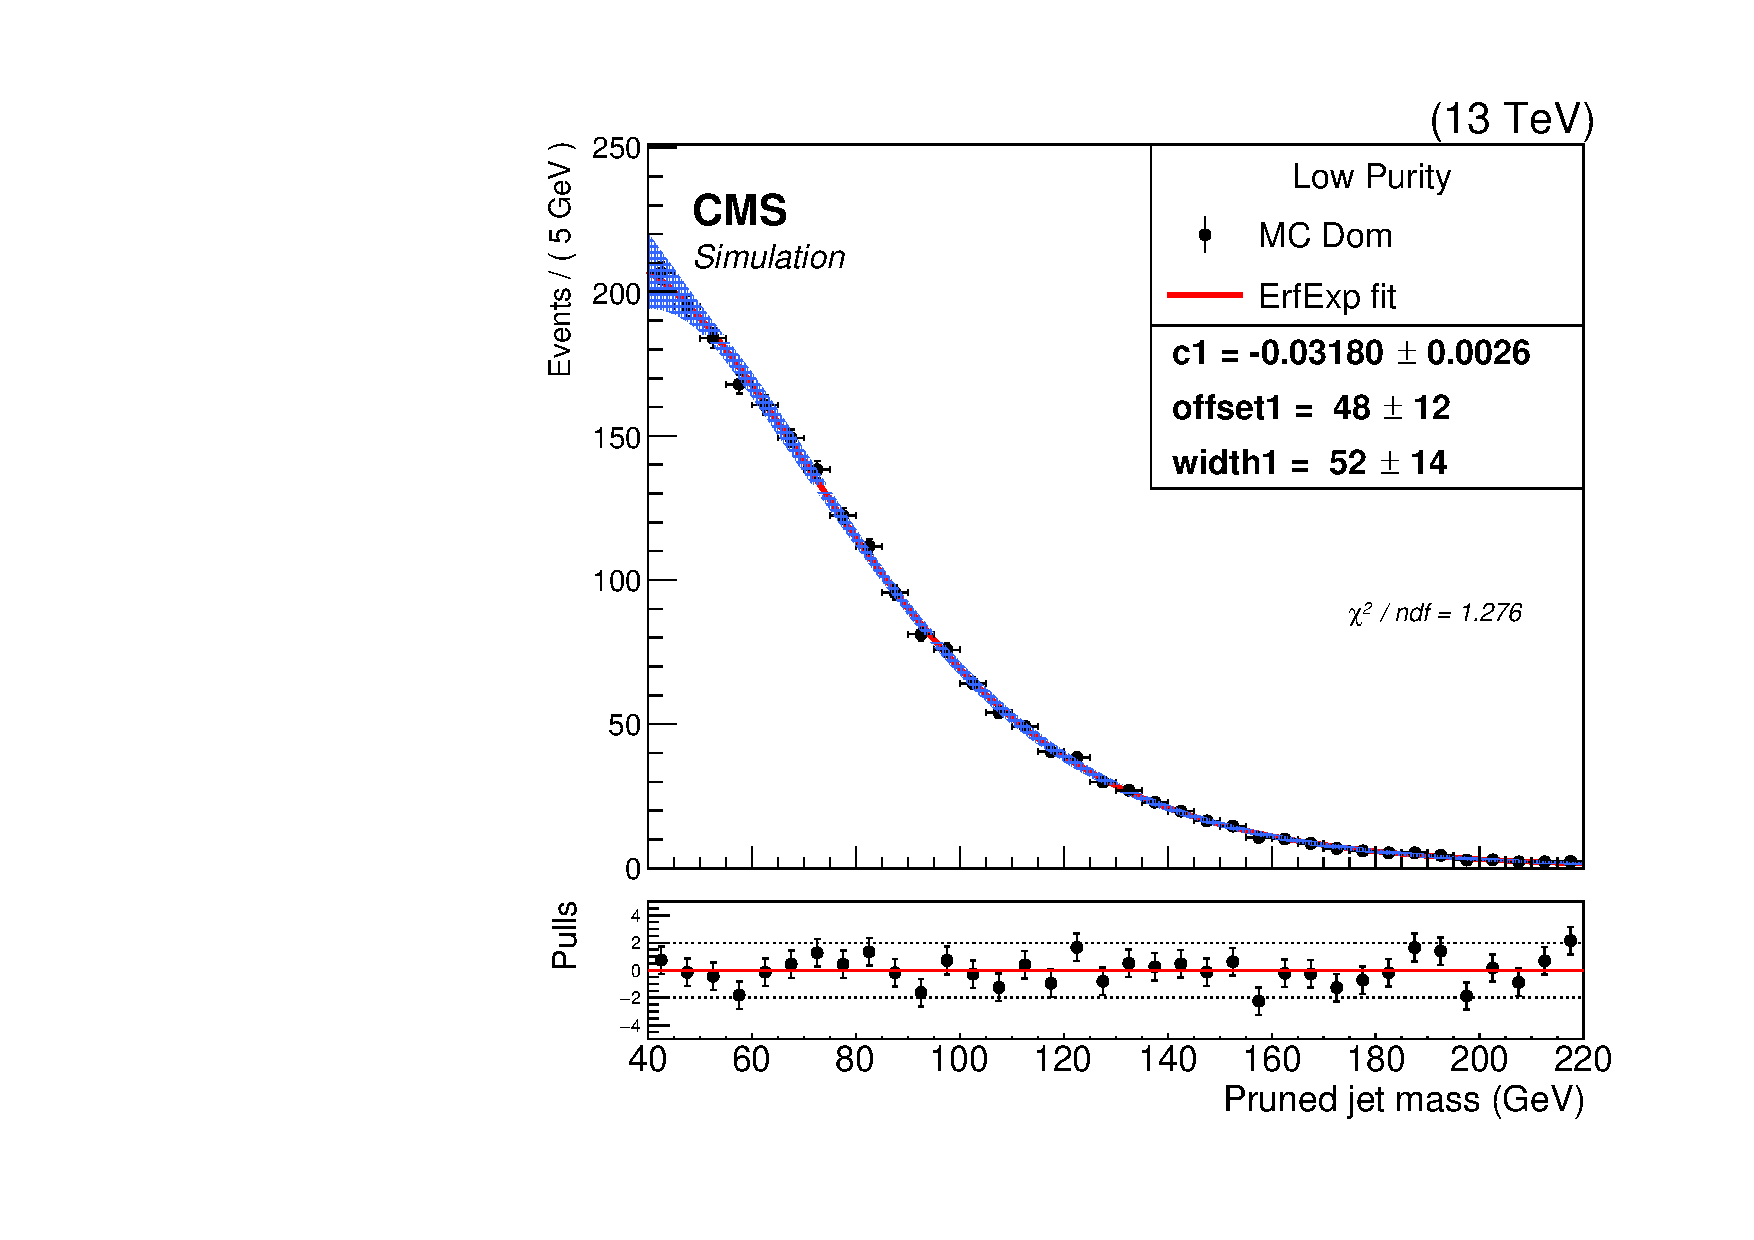
\includegraphics[width=250pt]{figuresARC/Vjets/DomLP.pdf} &
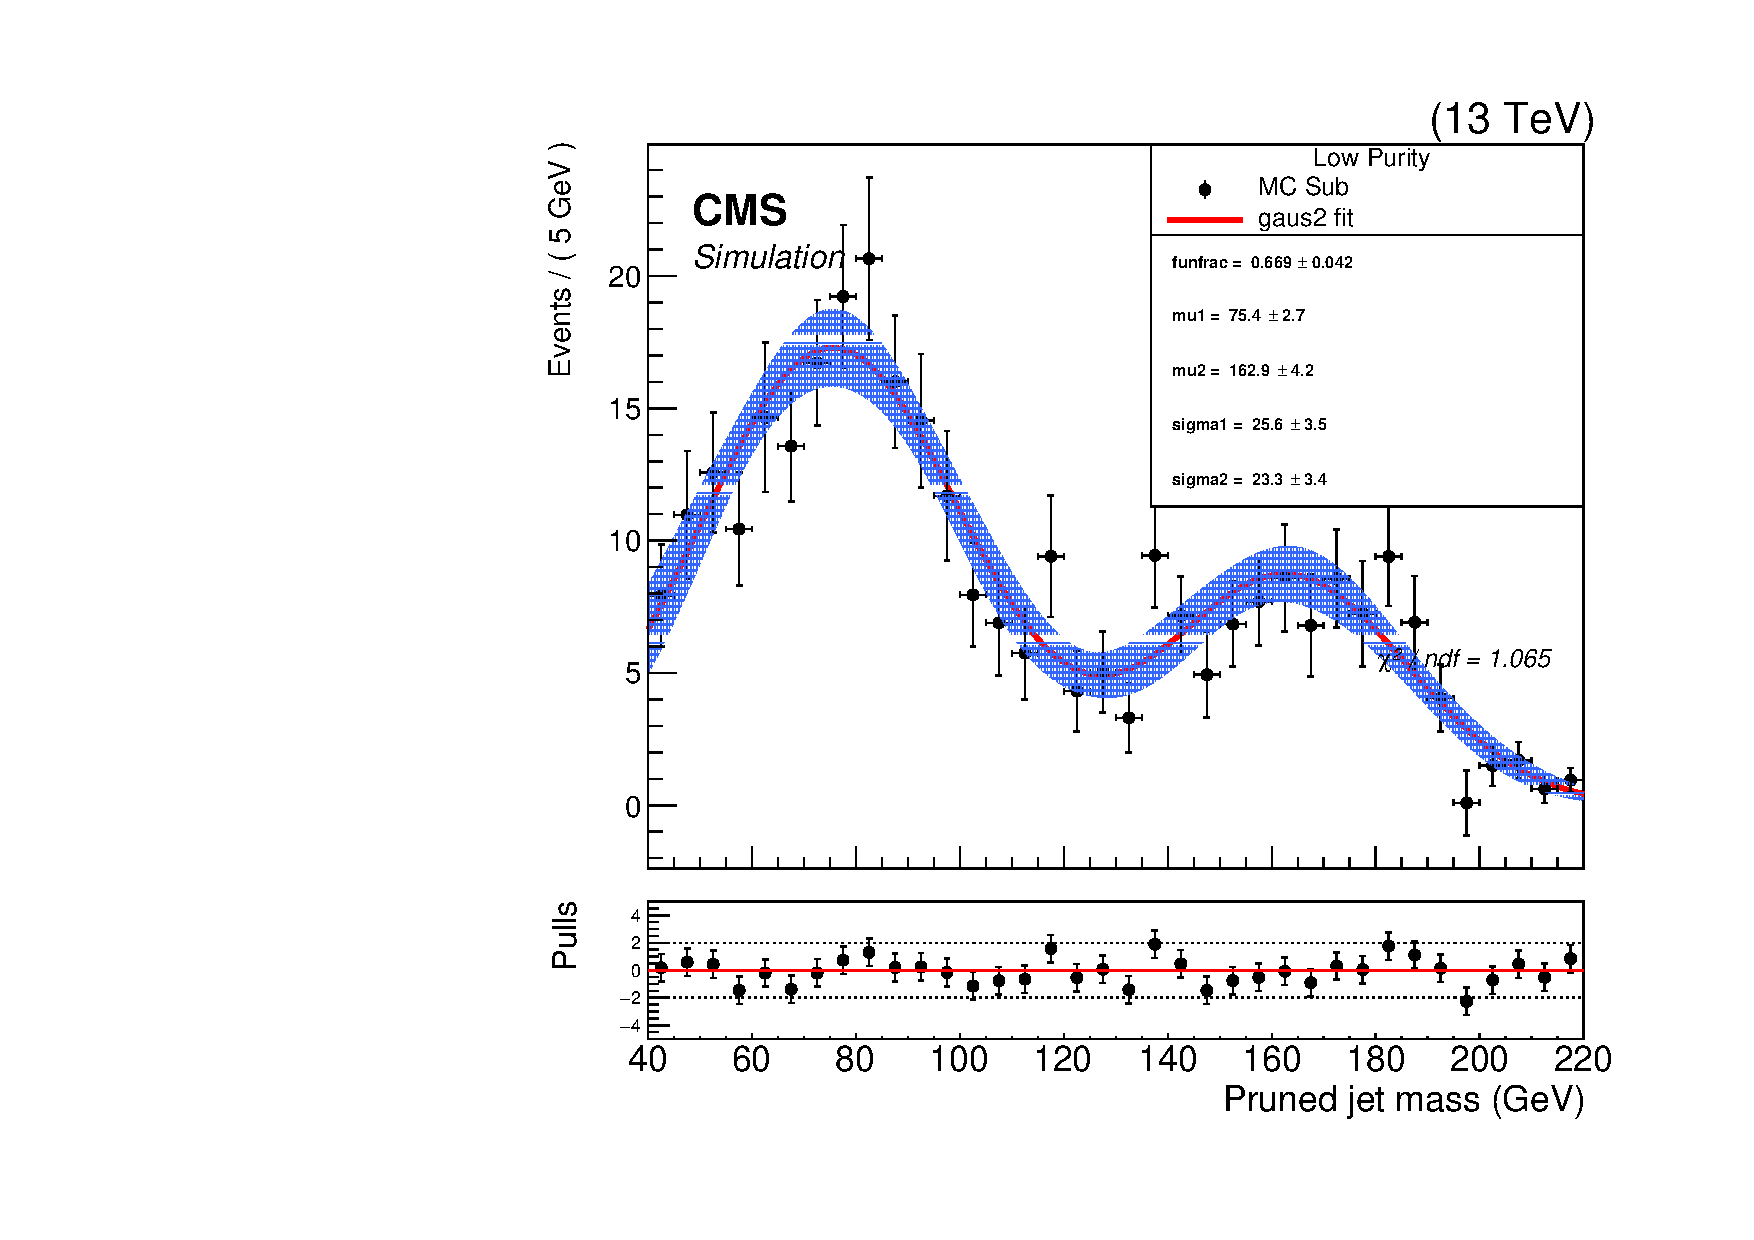
\includegraphics[width=250pt]{figuresARC/Vjets/SubDomLP.pdf}\\
\end{tabular}
\begin{center}
  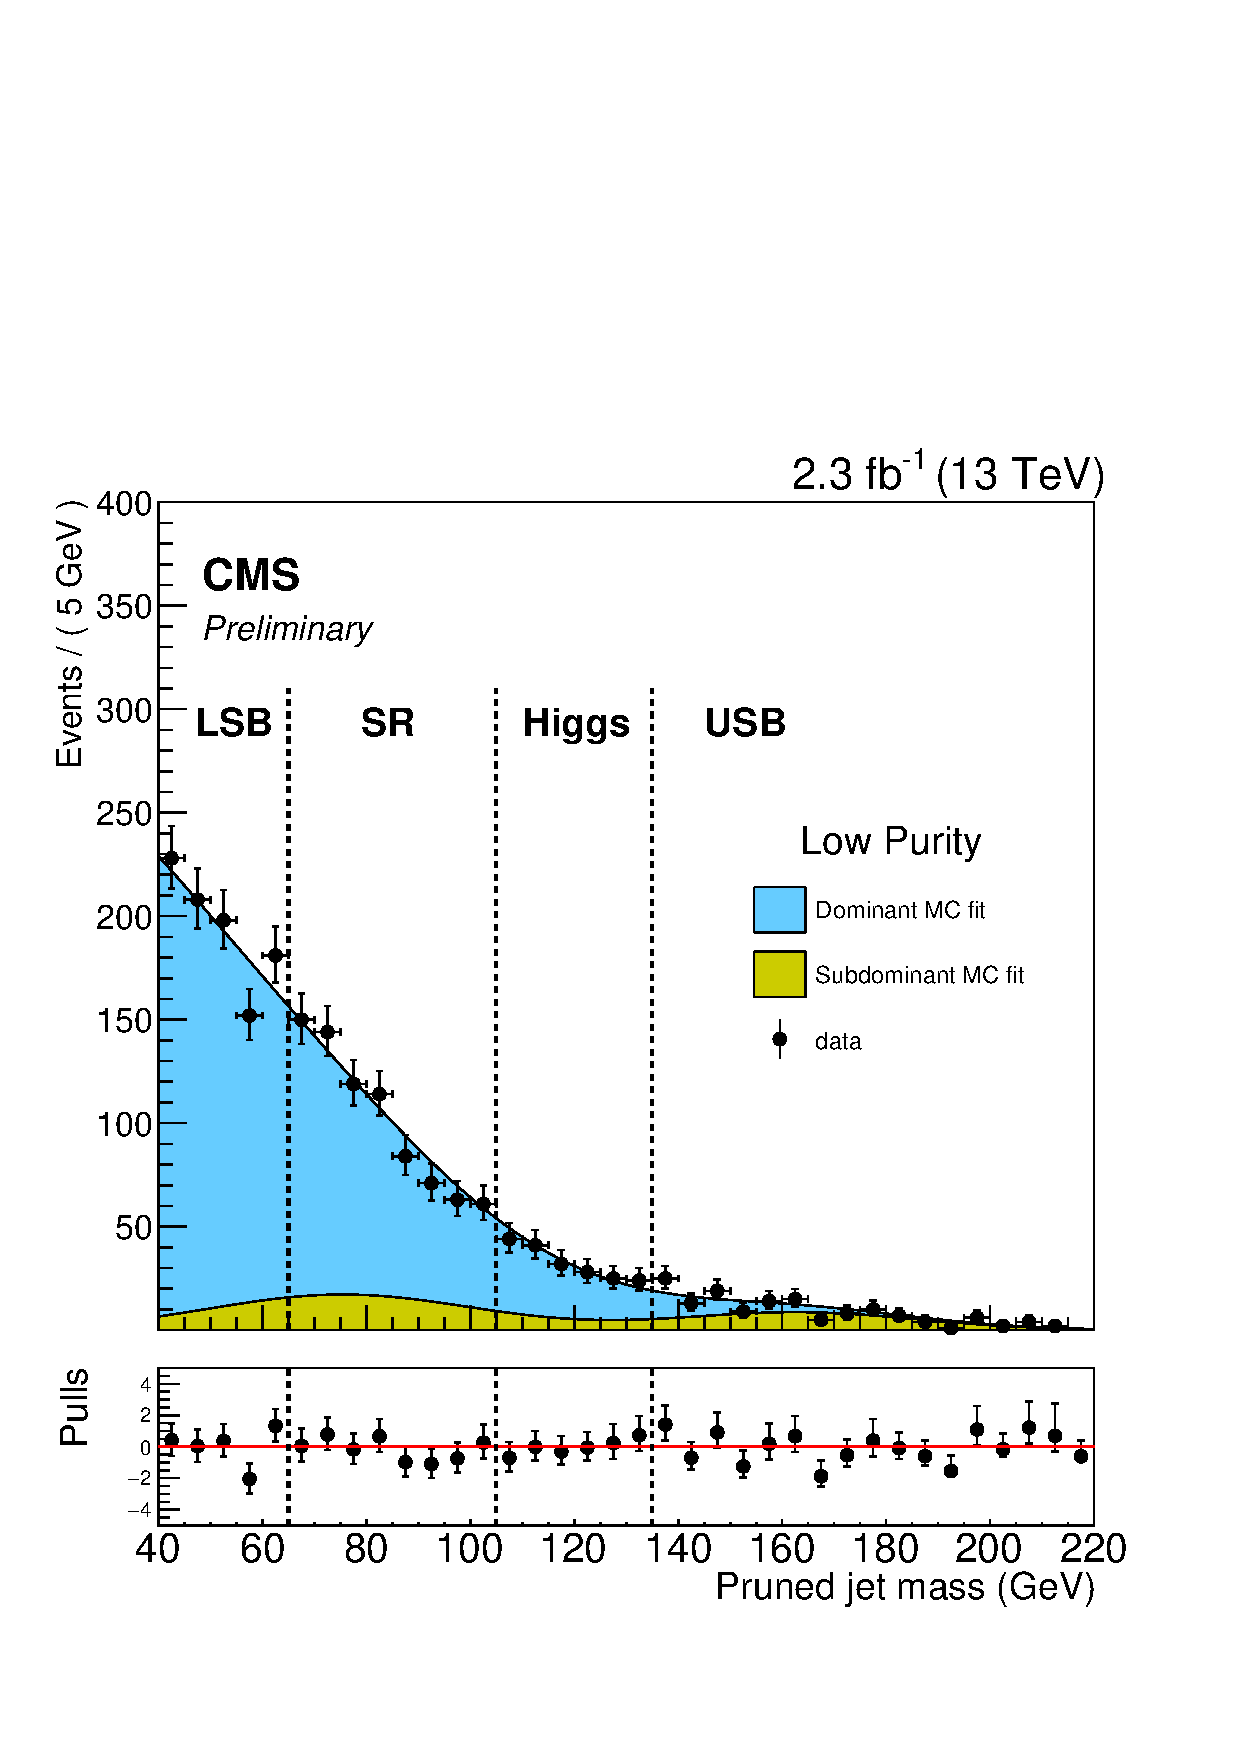
\includegraphics[width=270pt]{figuresARC/Vjets/dataMjUBLP.pdf}
\end{center}
\label{fig:fitprunedLP}
\end{figure}

\begin{figure}[!ht]
\caption{ Fit of the VZ candidate transverse mass in the HP category. Top: (left) Dominant MC background fit in the sideband region (right) Dominant MC background fit in the signal region. Center: (left) alpha transfer function (right) Data fit in the sideband region. Bottom: Final prediction on the background estimation in signal region.
The solid curve represents the background estimation provided by the data-driven
method. The hatched band includes both statistical and systematics uncertainties. The data
are shown as black markers. The bottom panels show the corresponding pull distributions,
quantifying the agreement between the background-only hypothesis and the data. The pull
distribution is defined as the difference between the data and the background prediction, divided by the error on data. The error bars on the points represent the error on data.
}
\begin{tabular}{cc}
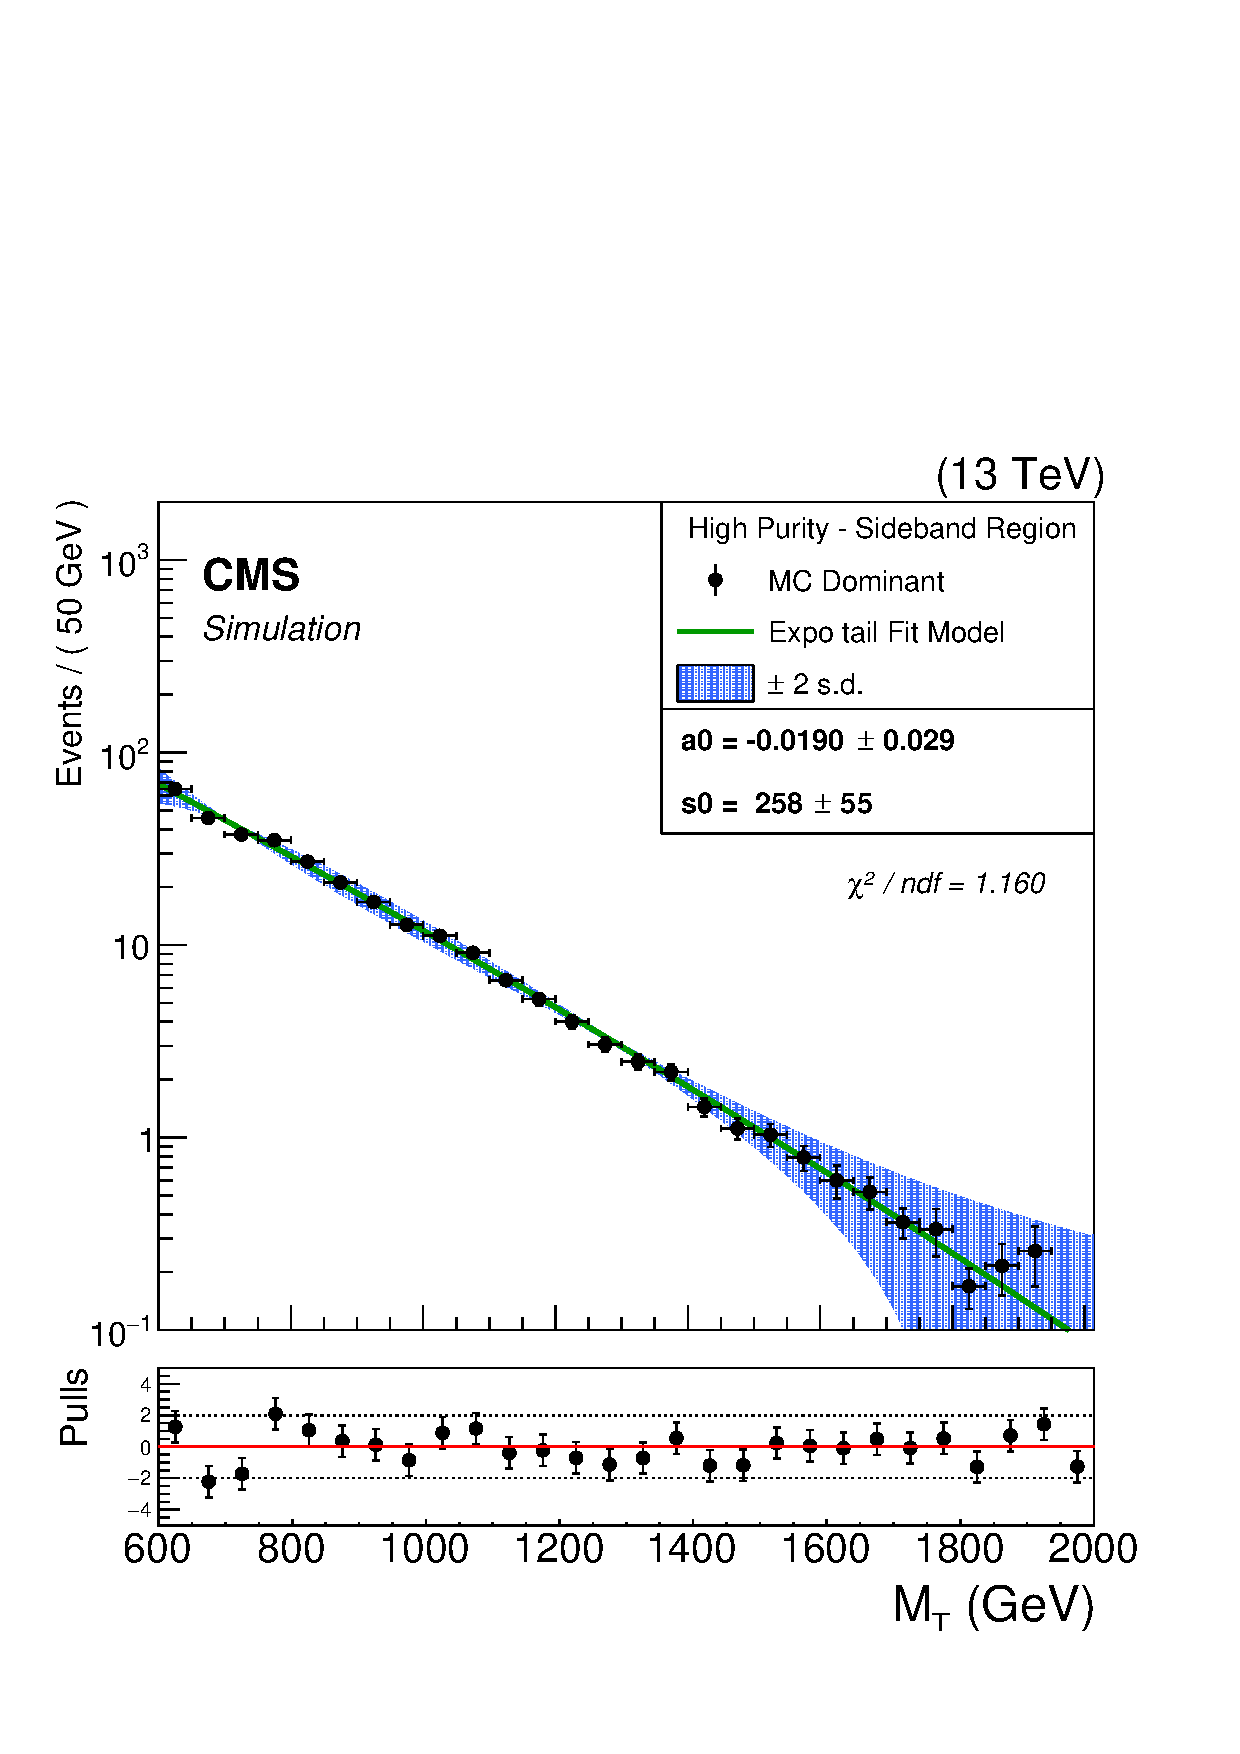
\includegraphics[width=150pt]{figuresARC/fits/sbDom_MVZHP.pdf} &
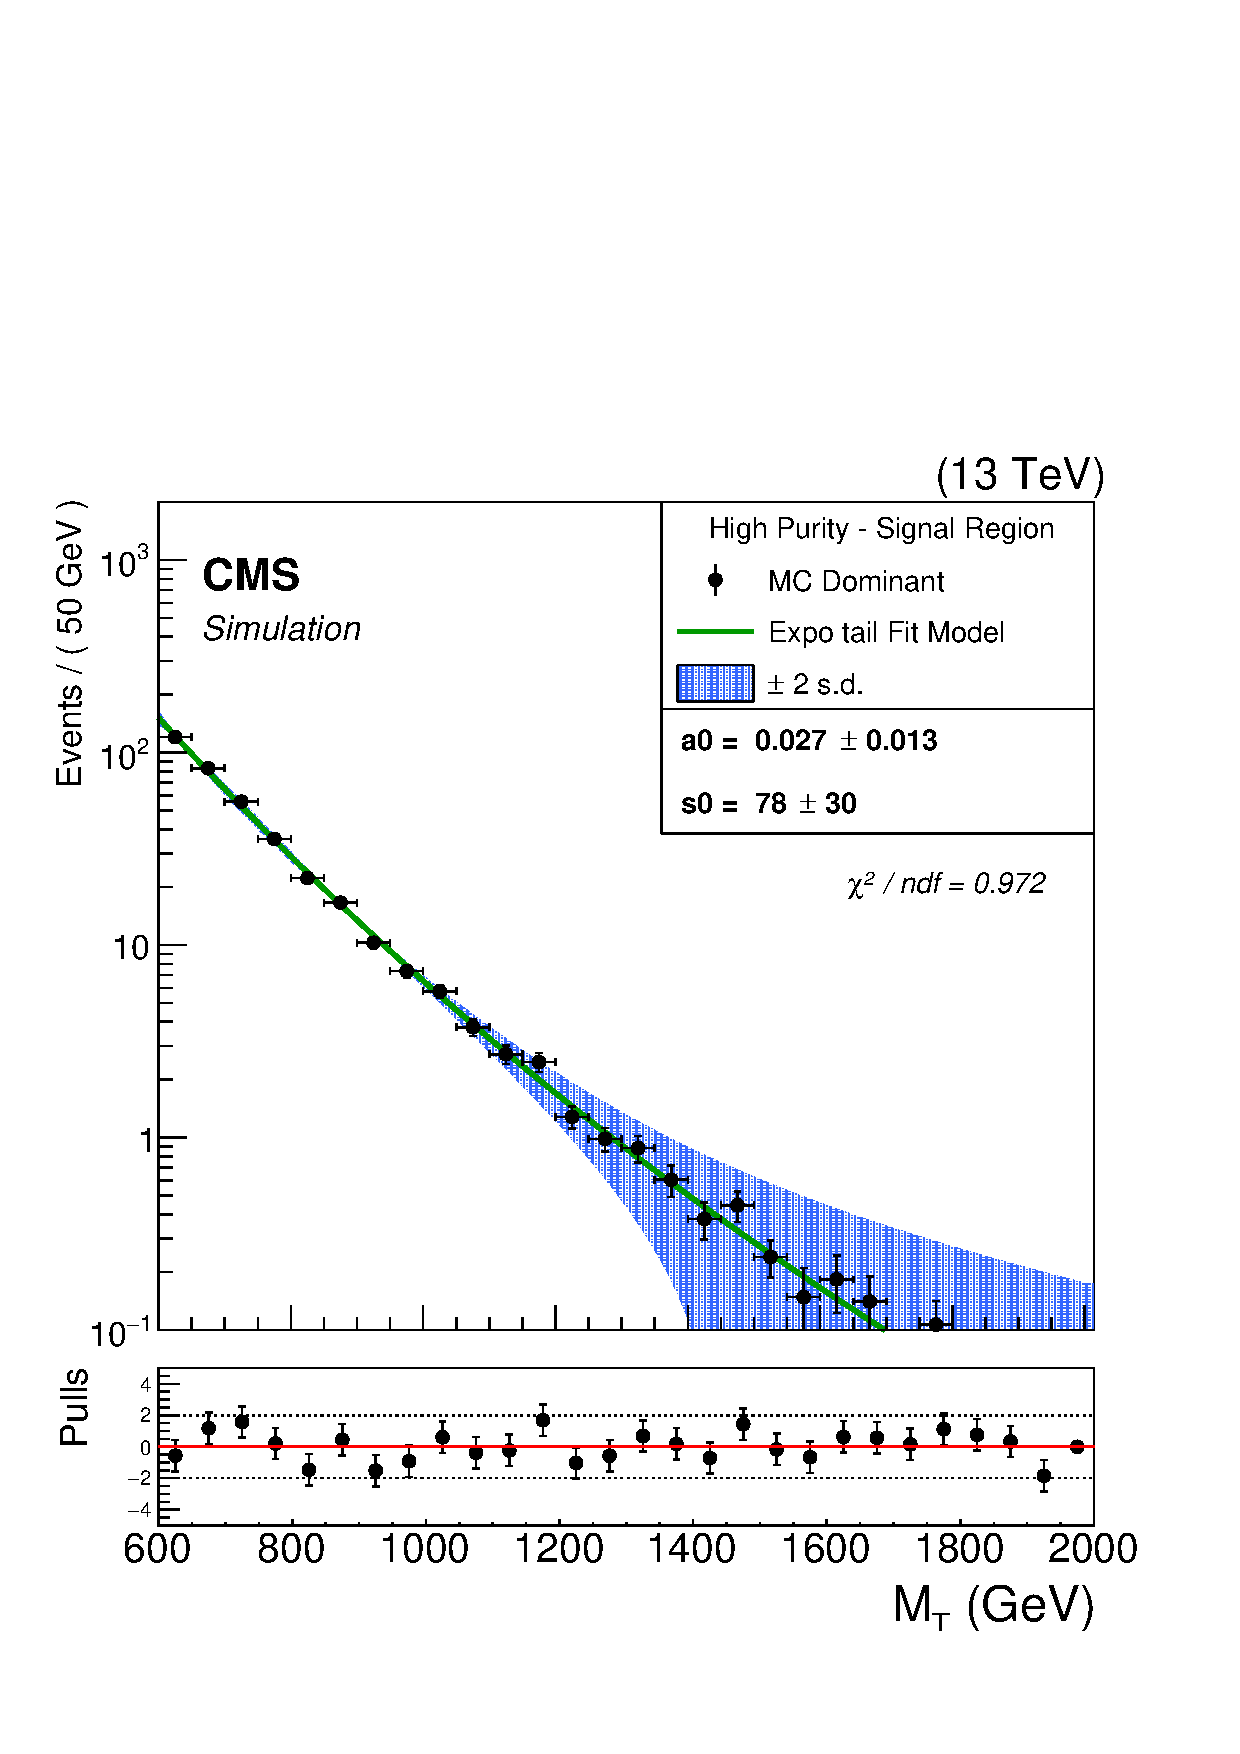
\includegraphics[width=150pt]{figuresARC/fits/sigDom_MVZHP.pdf}\\
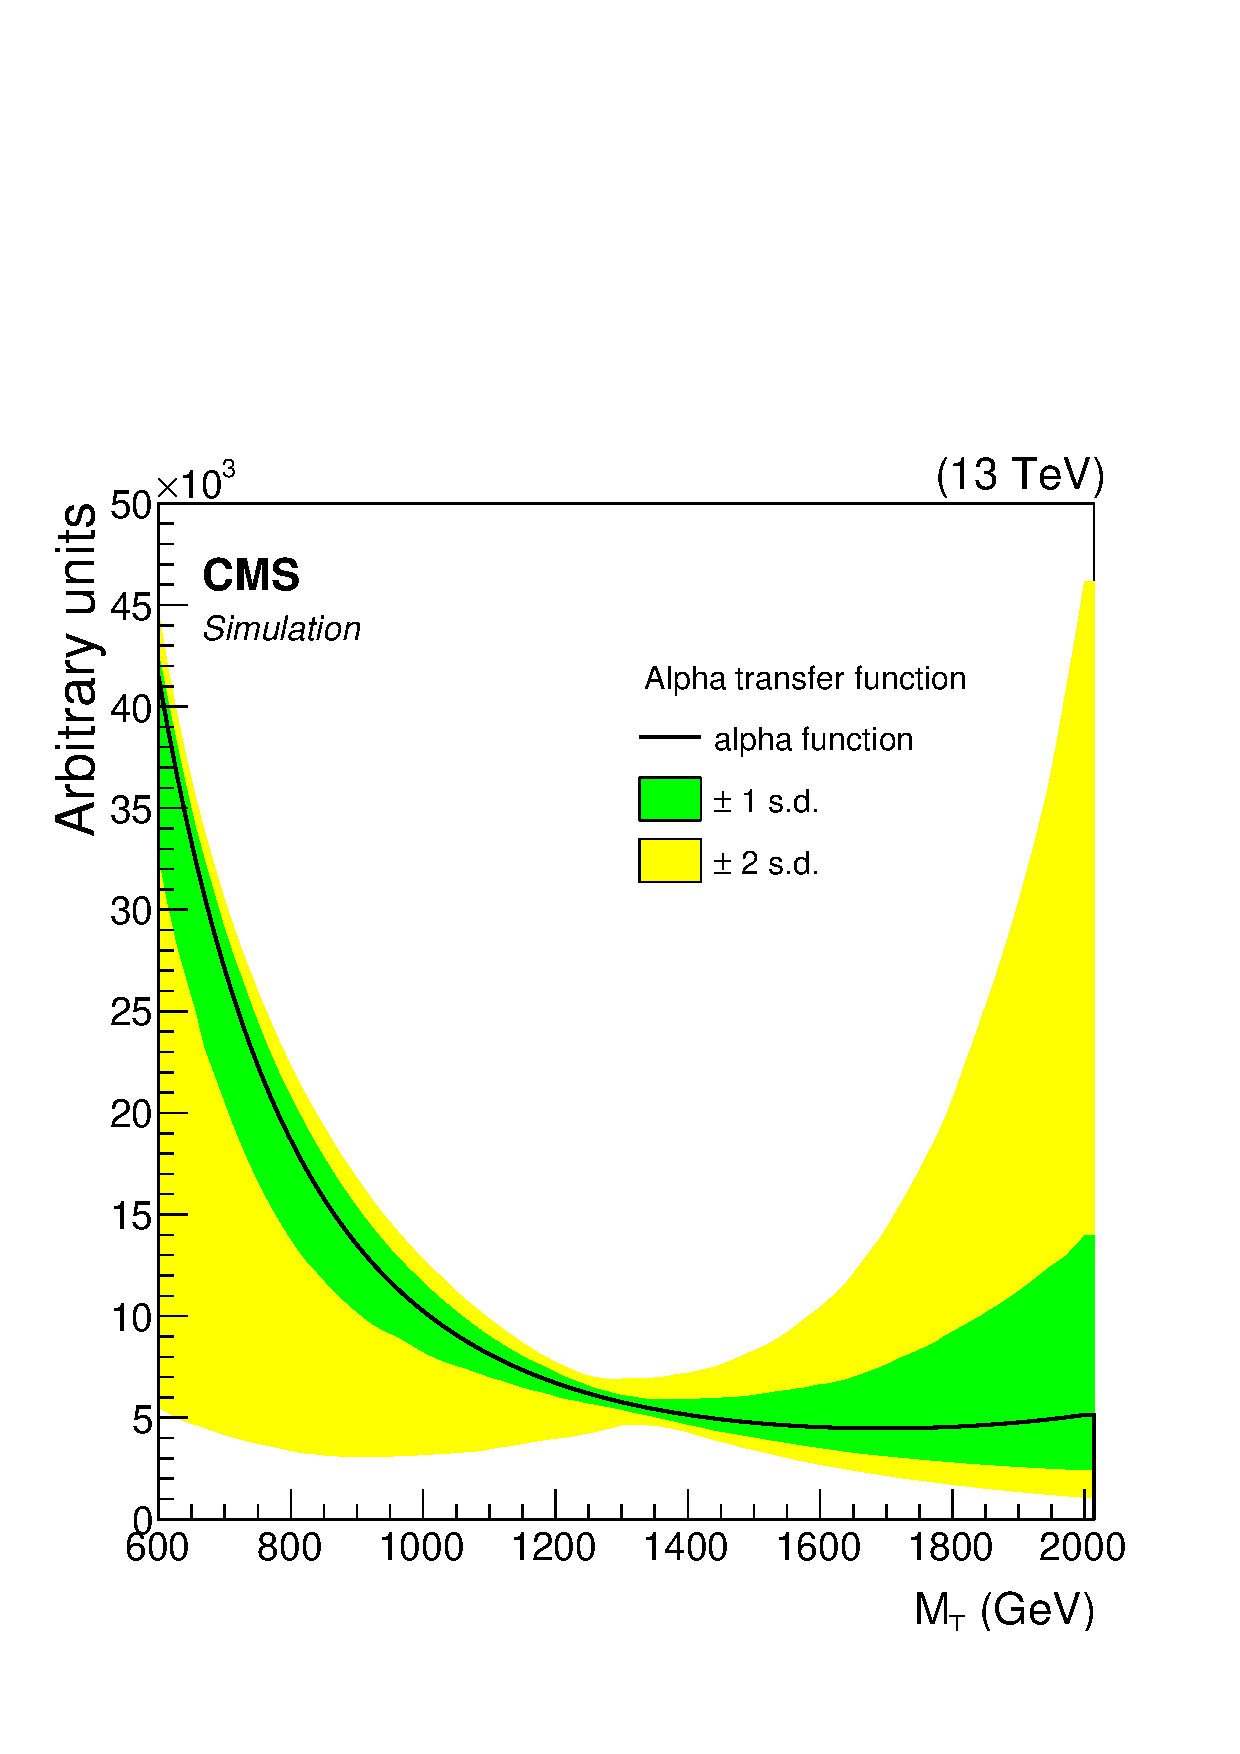
\includegraphics[width=150pt]{figuresARC/fits/alphaHP.pdf}&
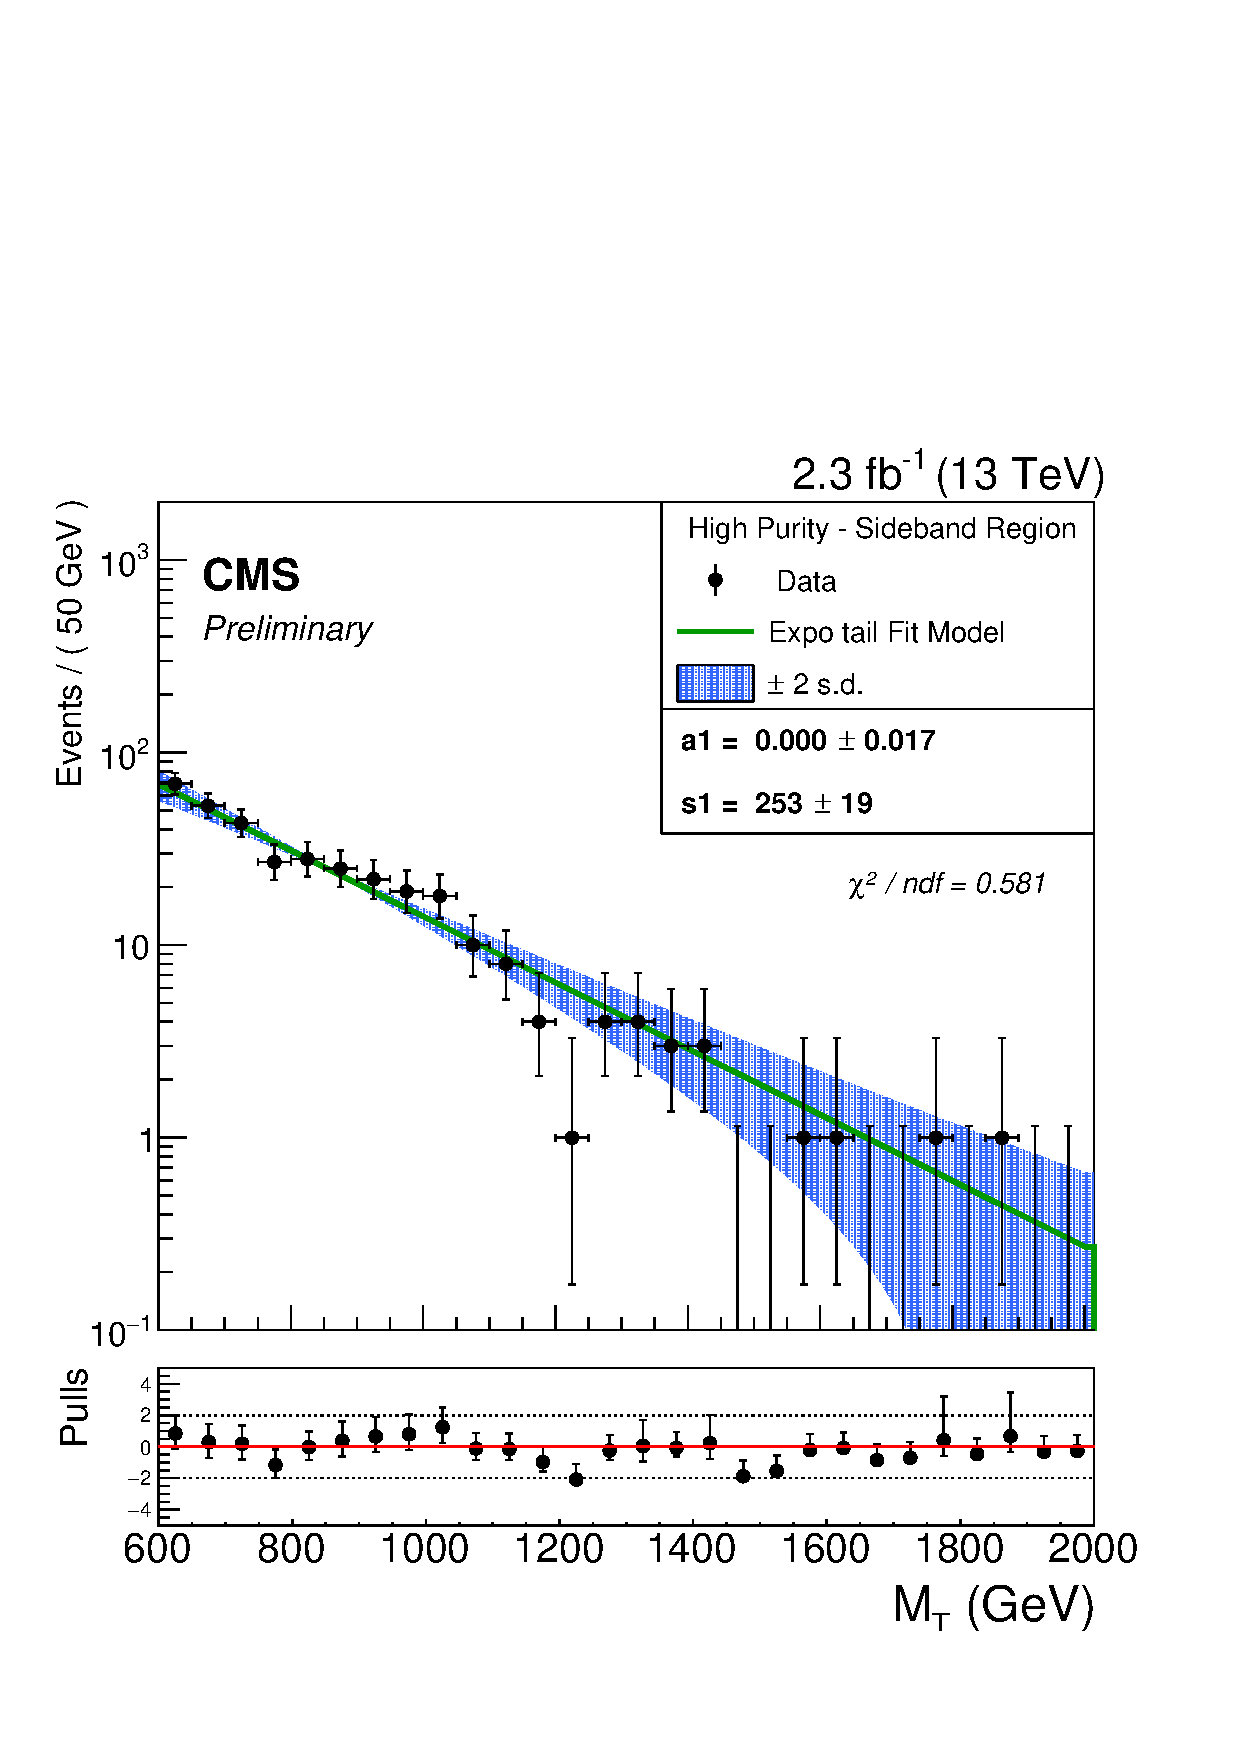
\includegraphics[width=150pt]{figuresARC/fits/sbData_MVZHP.pdf}\\
\end{tabular}
\begin{center}
  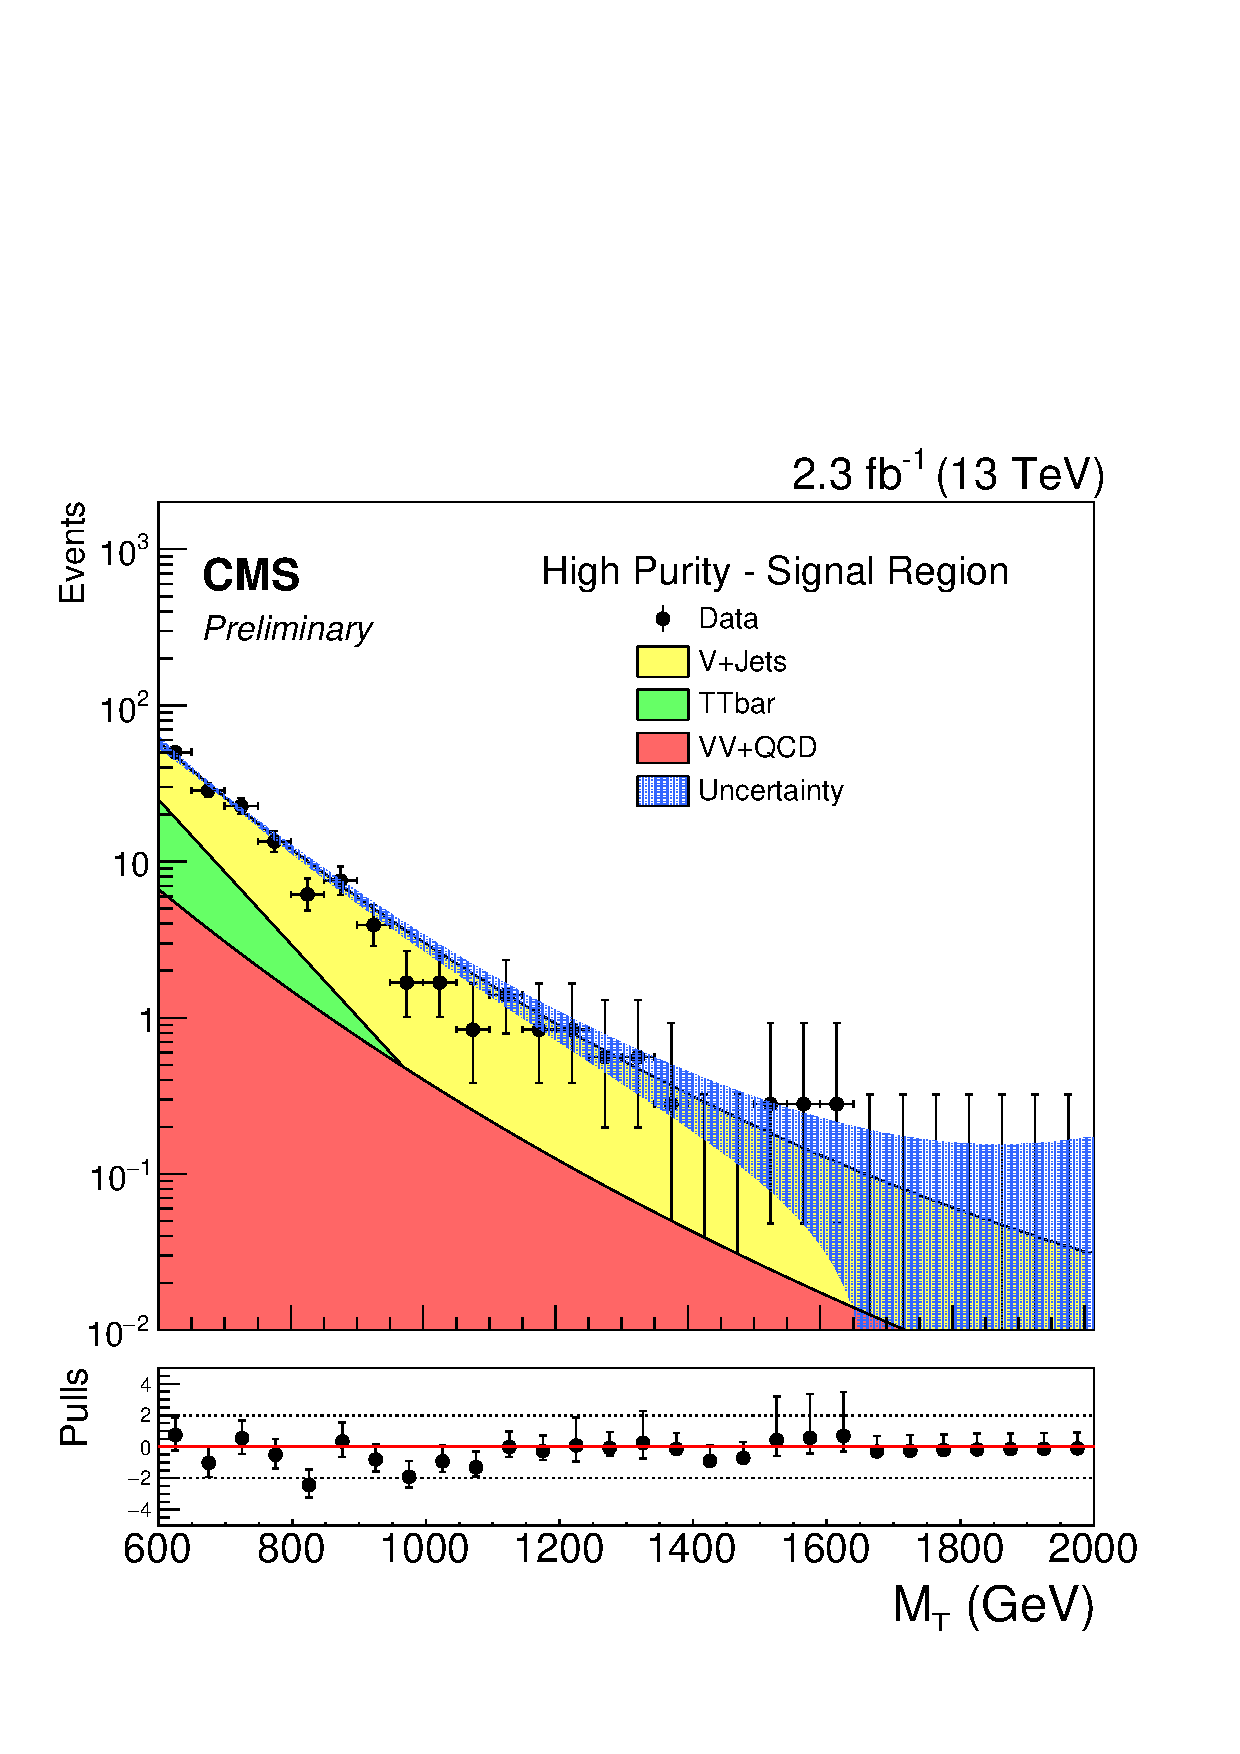
\includegraphics[width=200pt]{figuresARC/fits/finalresultUBHP.pdf}
\end{center}
\label{fig:fits3}
\end{figure}


\begin{figure}[!ht]
\caption{ Fit of the VZ candidate transverse mass in the LP category. Top: (left) Dominant MC background fit in the sideband region (right) Dominant MC background fit in the signal region. Center: (left) alpha transfer function (right) Data fit in the sideband region. Bottom: Final prediction on the background estimation in signal region.
The solid curve represents the background estimation provided by the data-driven
method. The hatched band includes both statistical and systematics uncertainties. The data
are shown as black markers. The bottom panels show the corresponding pull distributions,
quantifying the agreement between the background-only hypothesis and the data. The pull
distribution is defined as the difference between the data and the background prediction, divided by the error on data. The error bars on the points represent the error on data.}
\begin{tabular}{cc}
  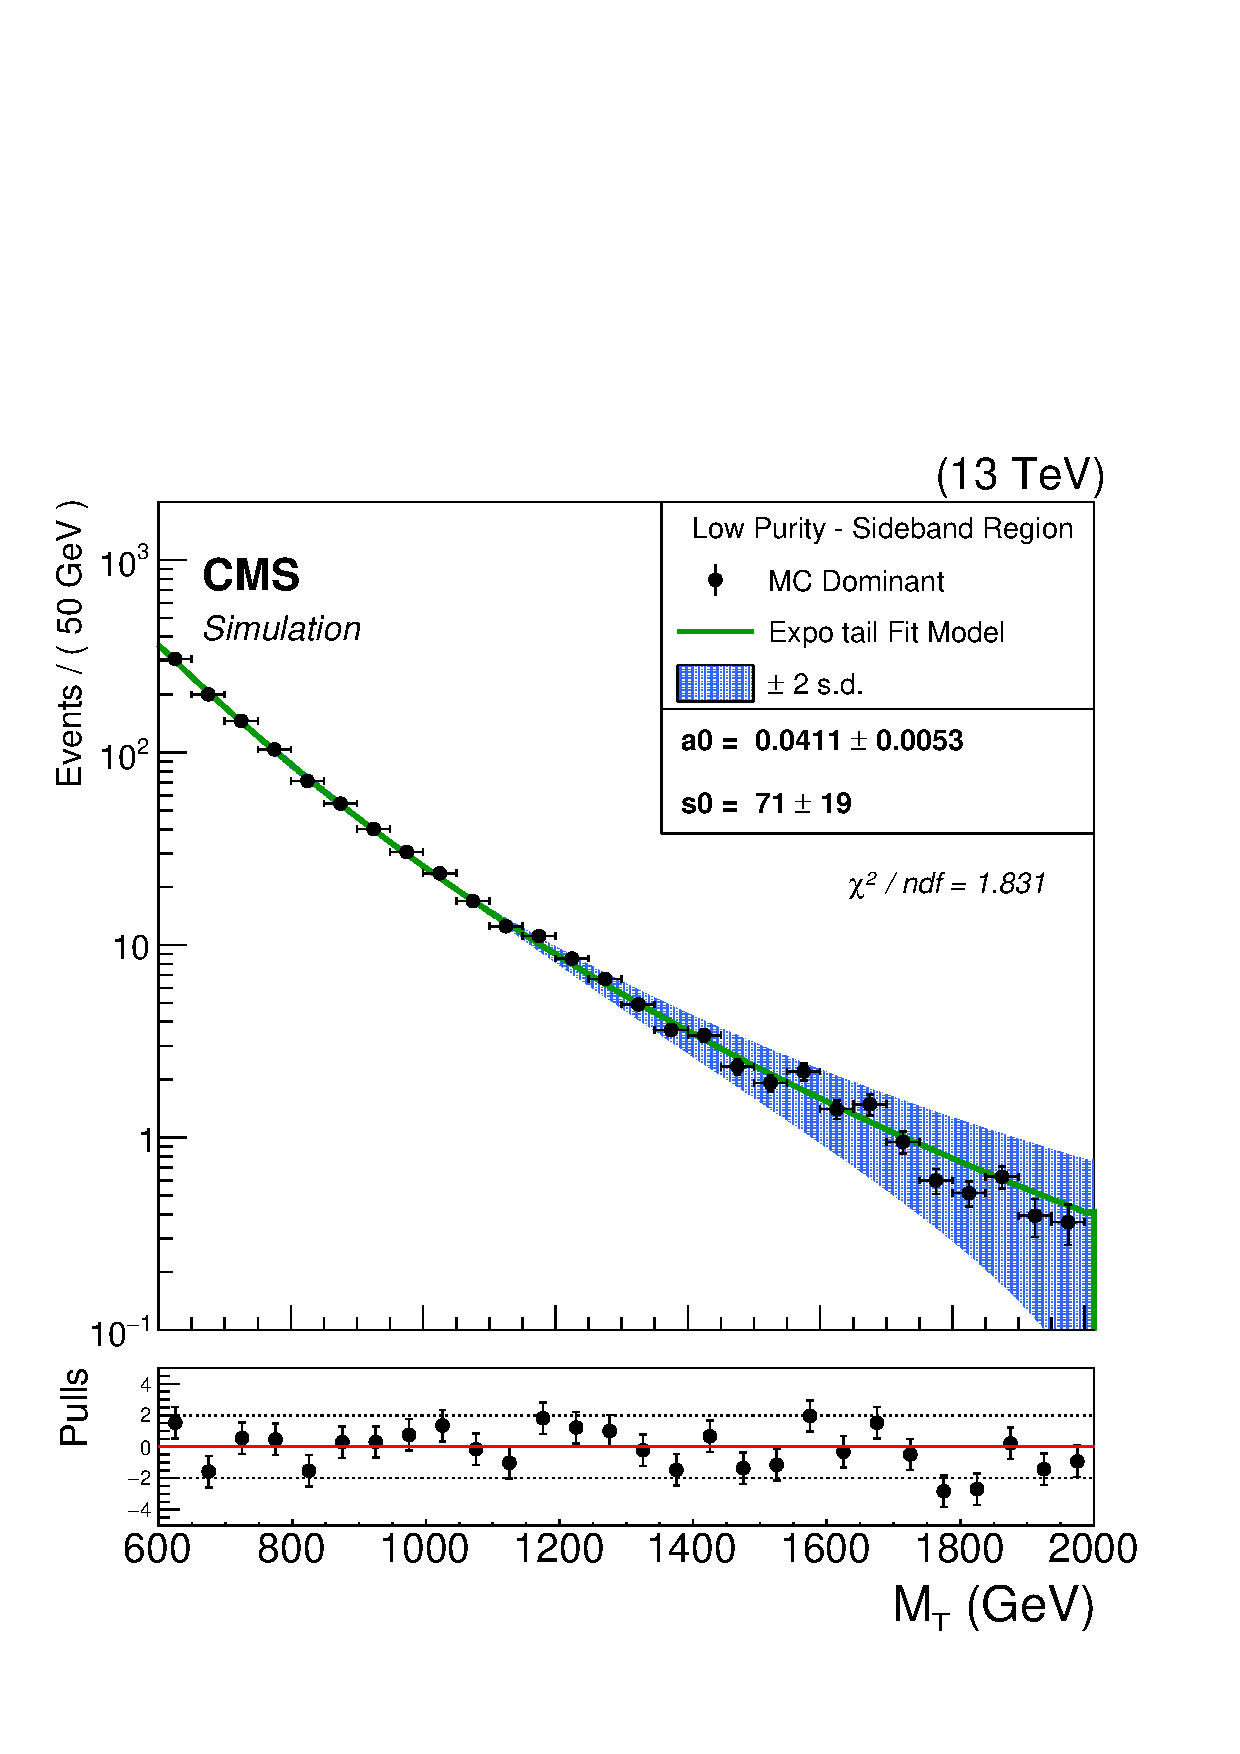
\includegraphics[width=150pt]{figuresARC/fits/sbDom_MVZLP.pdf} &
  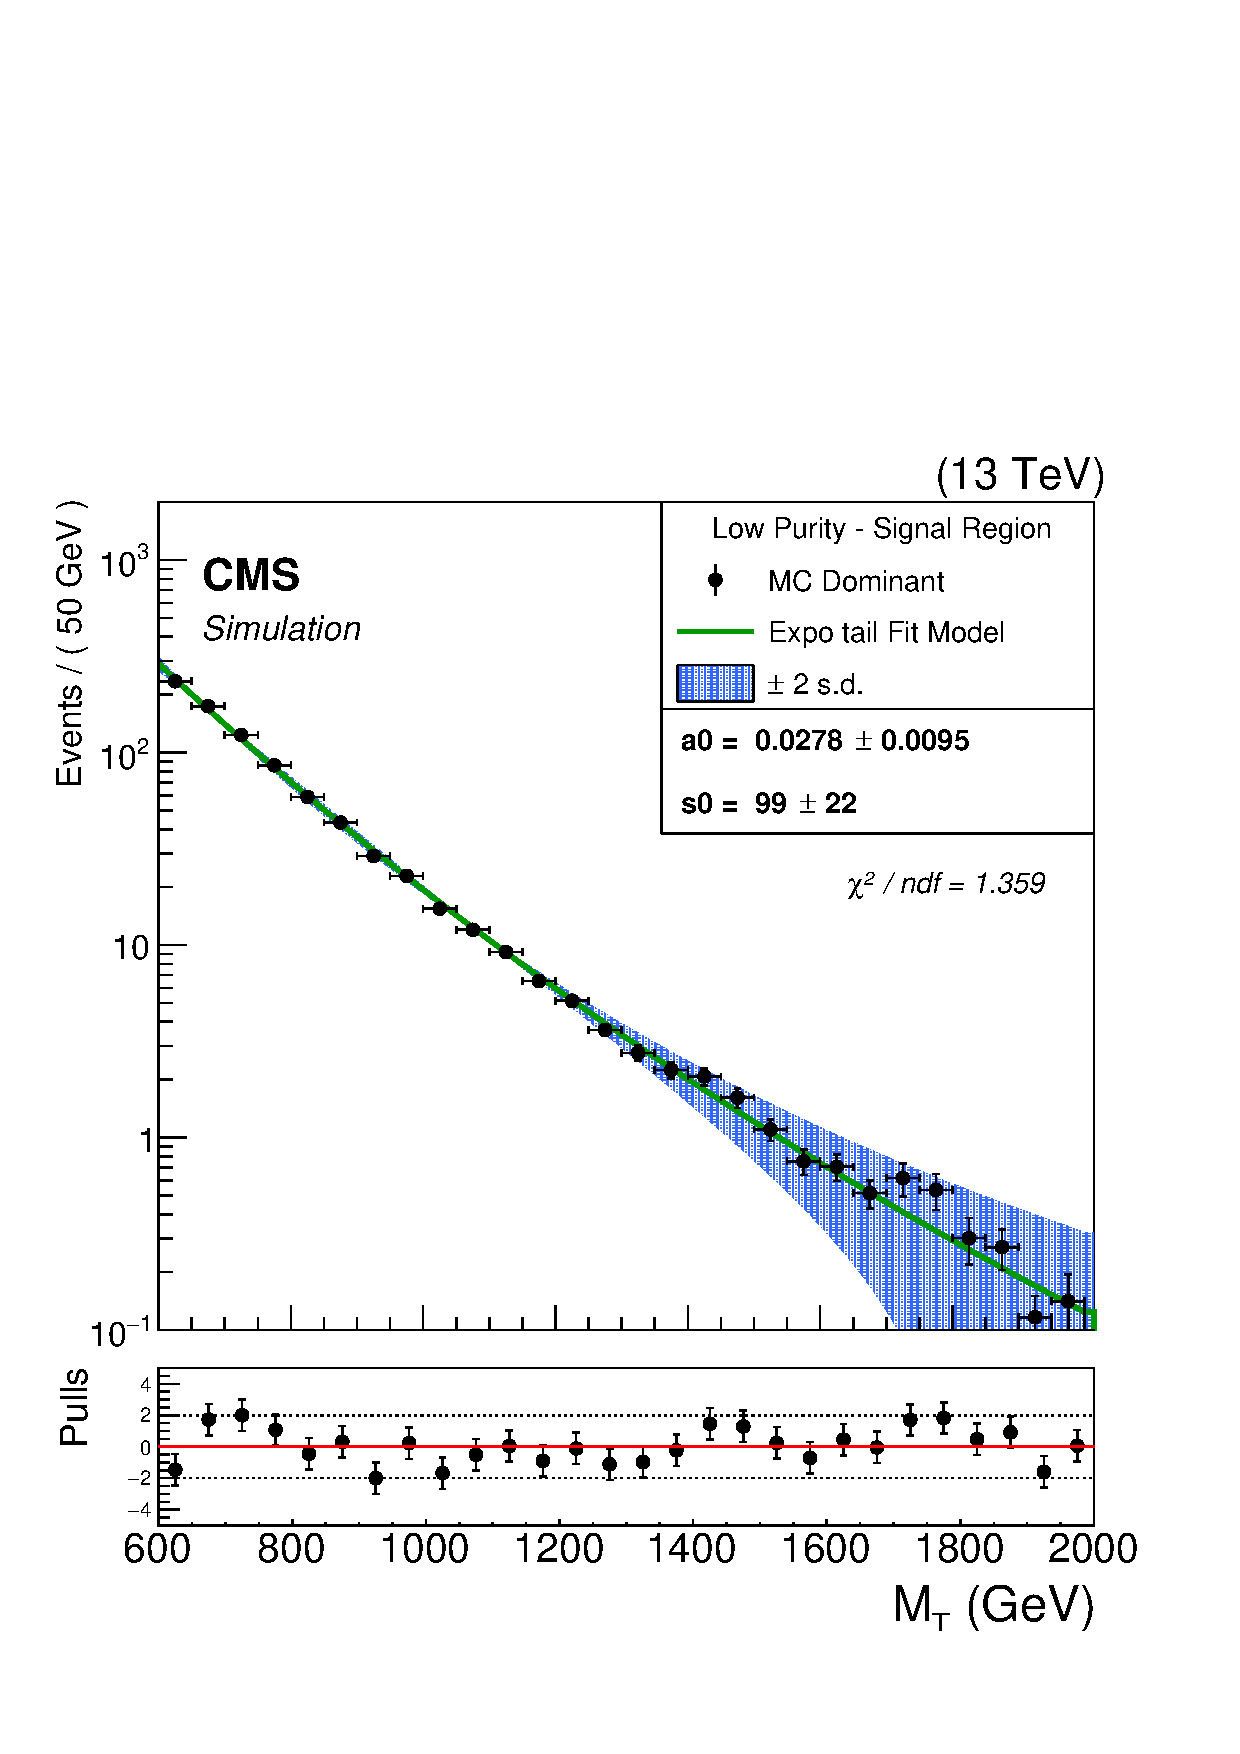
\includegraphics[width=150pt]{figuresARC/fits/sigDom_MVZLP.pdf}\\
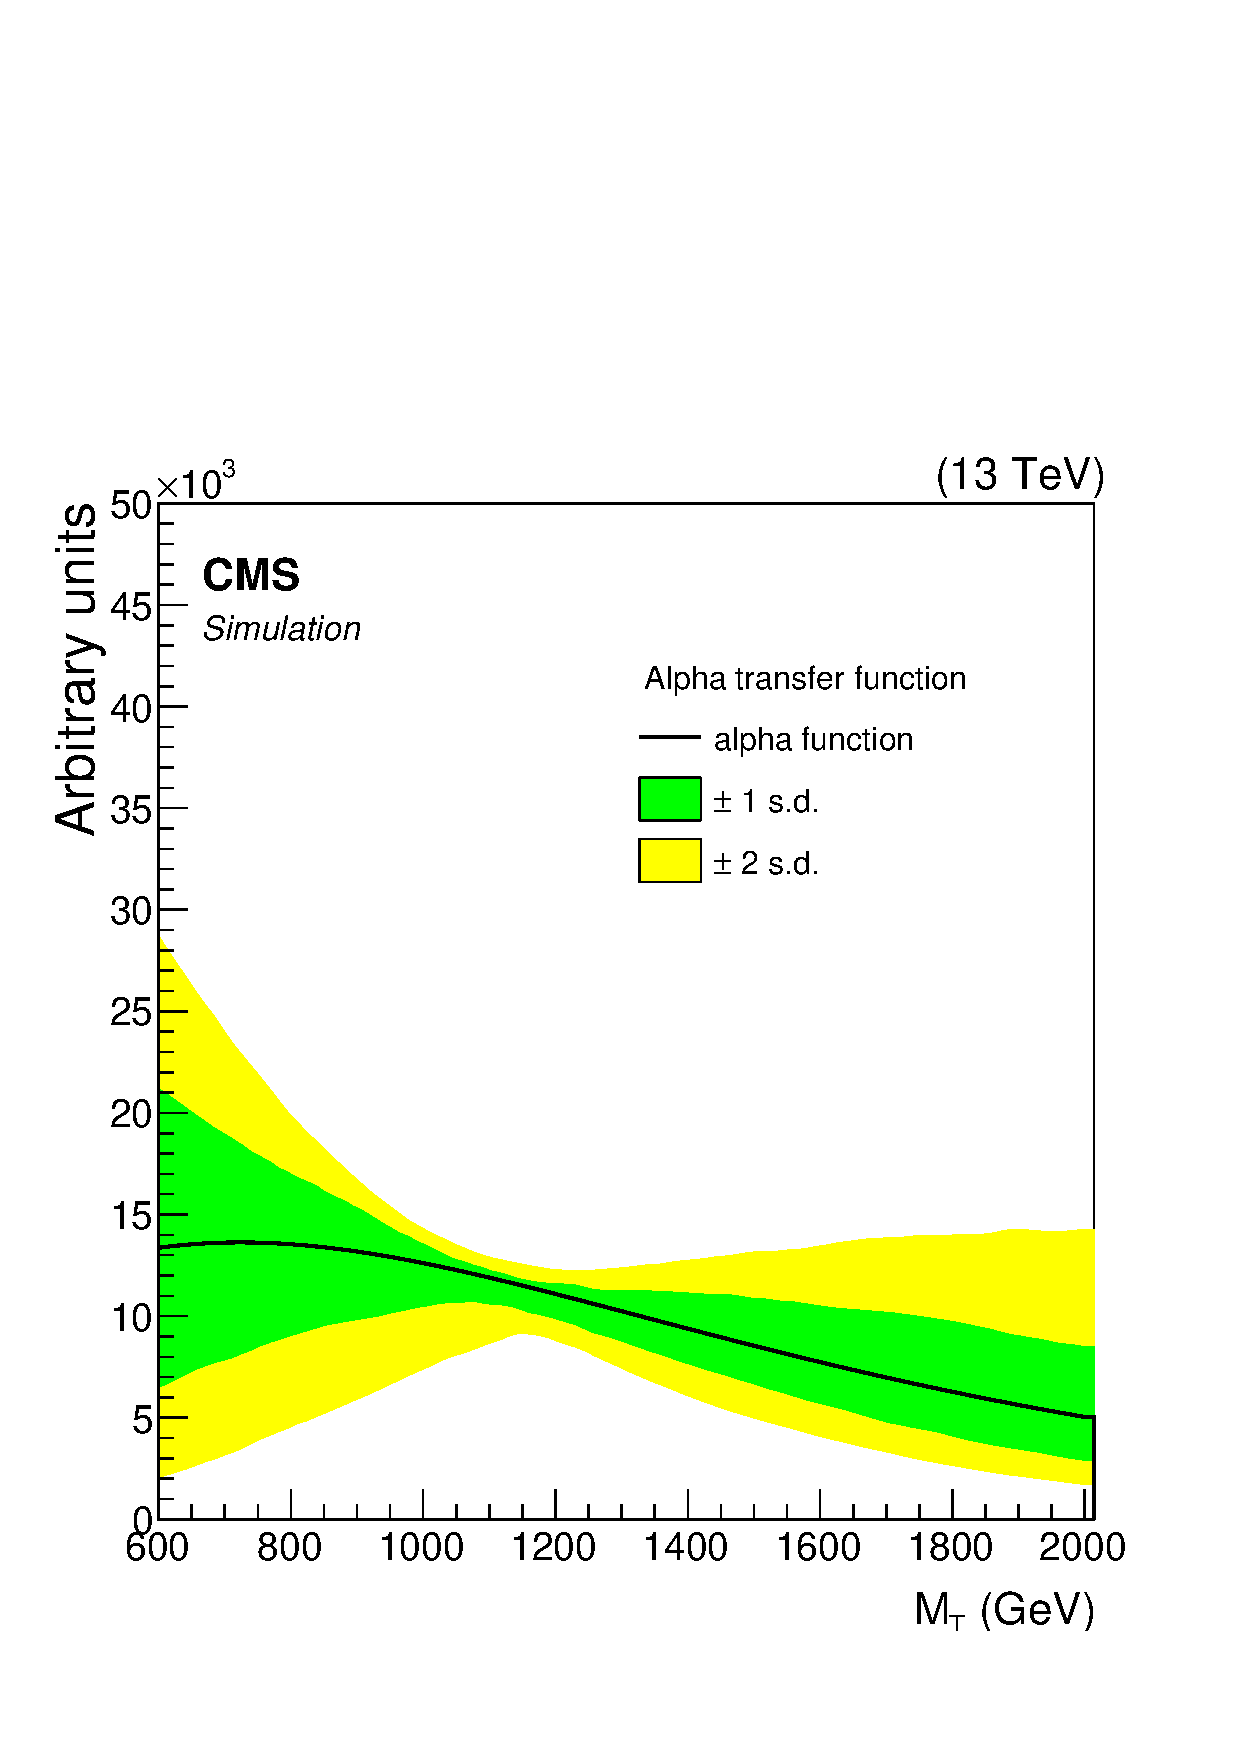
\includegraphics[width=150pt]{figuresARC/fits/alphaLP.pdf}&
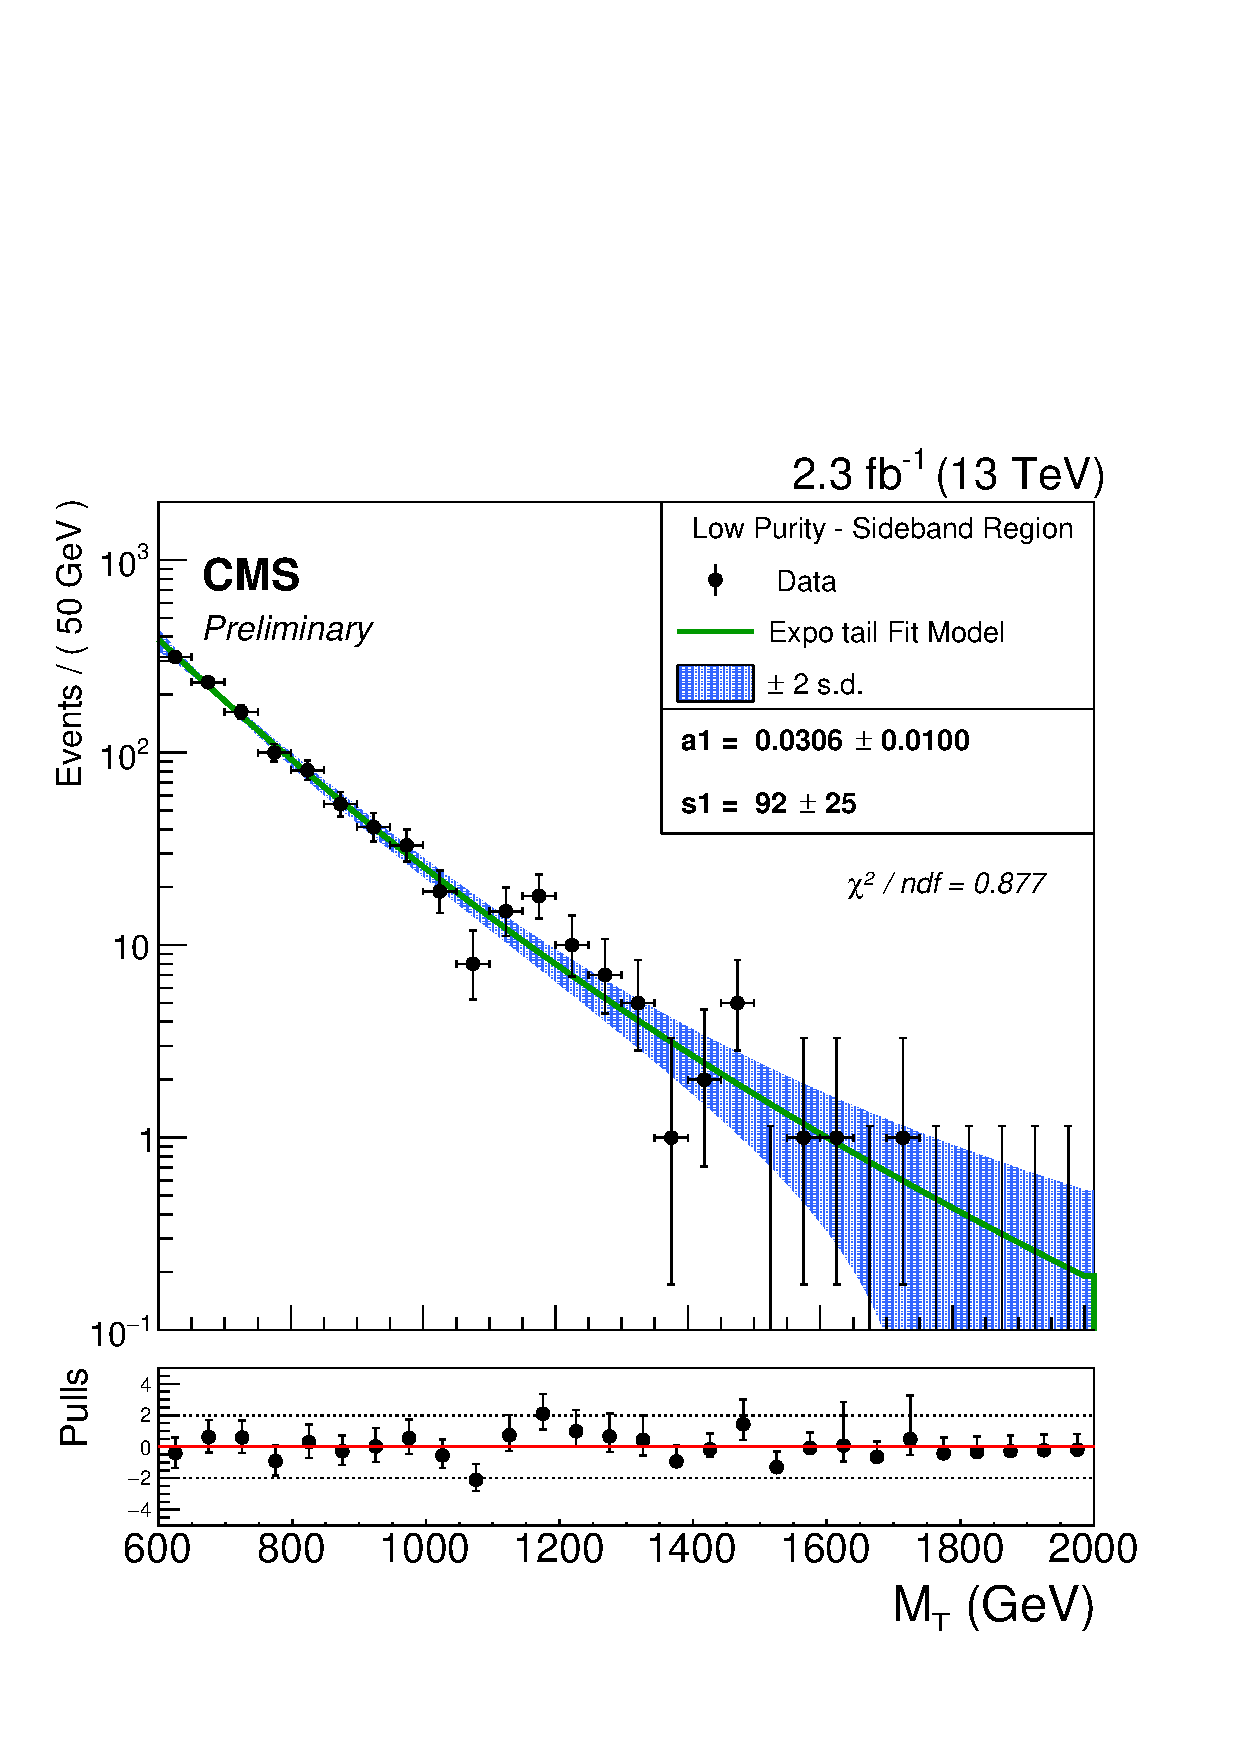
\includegraphics[width=150pt]{figuresARC/fits/sbData_MVZLP.pdf}\\
\end{tabular}
\begin{center}
  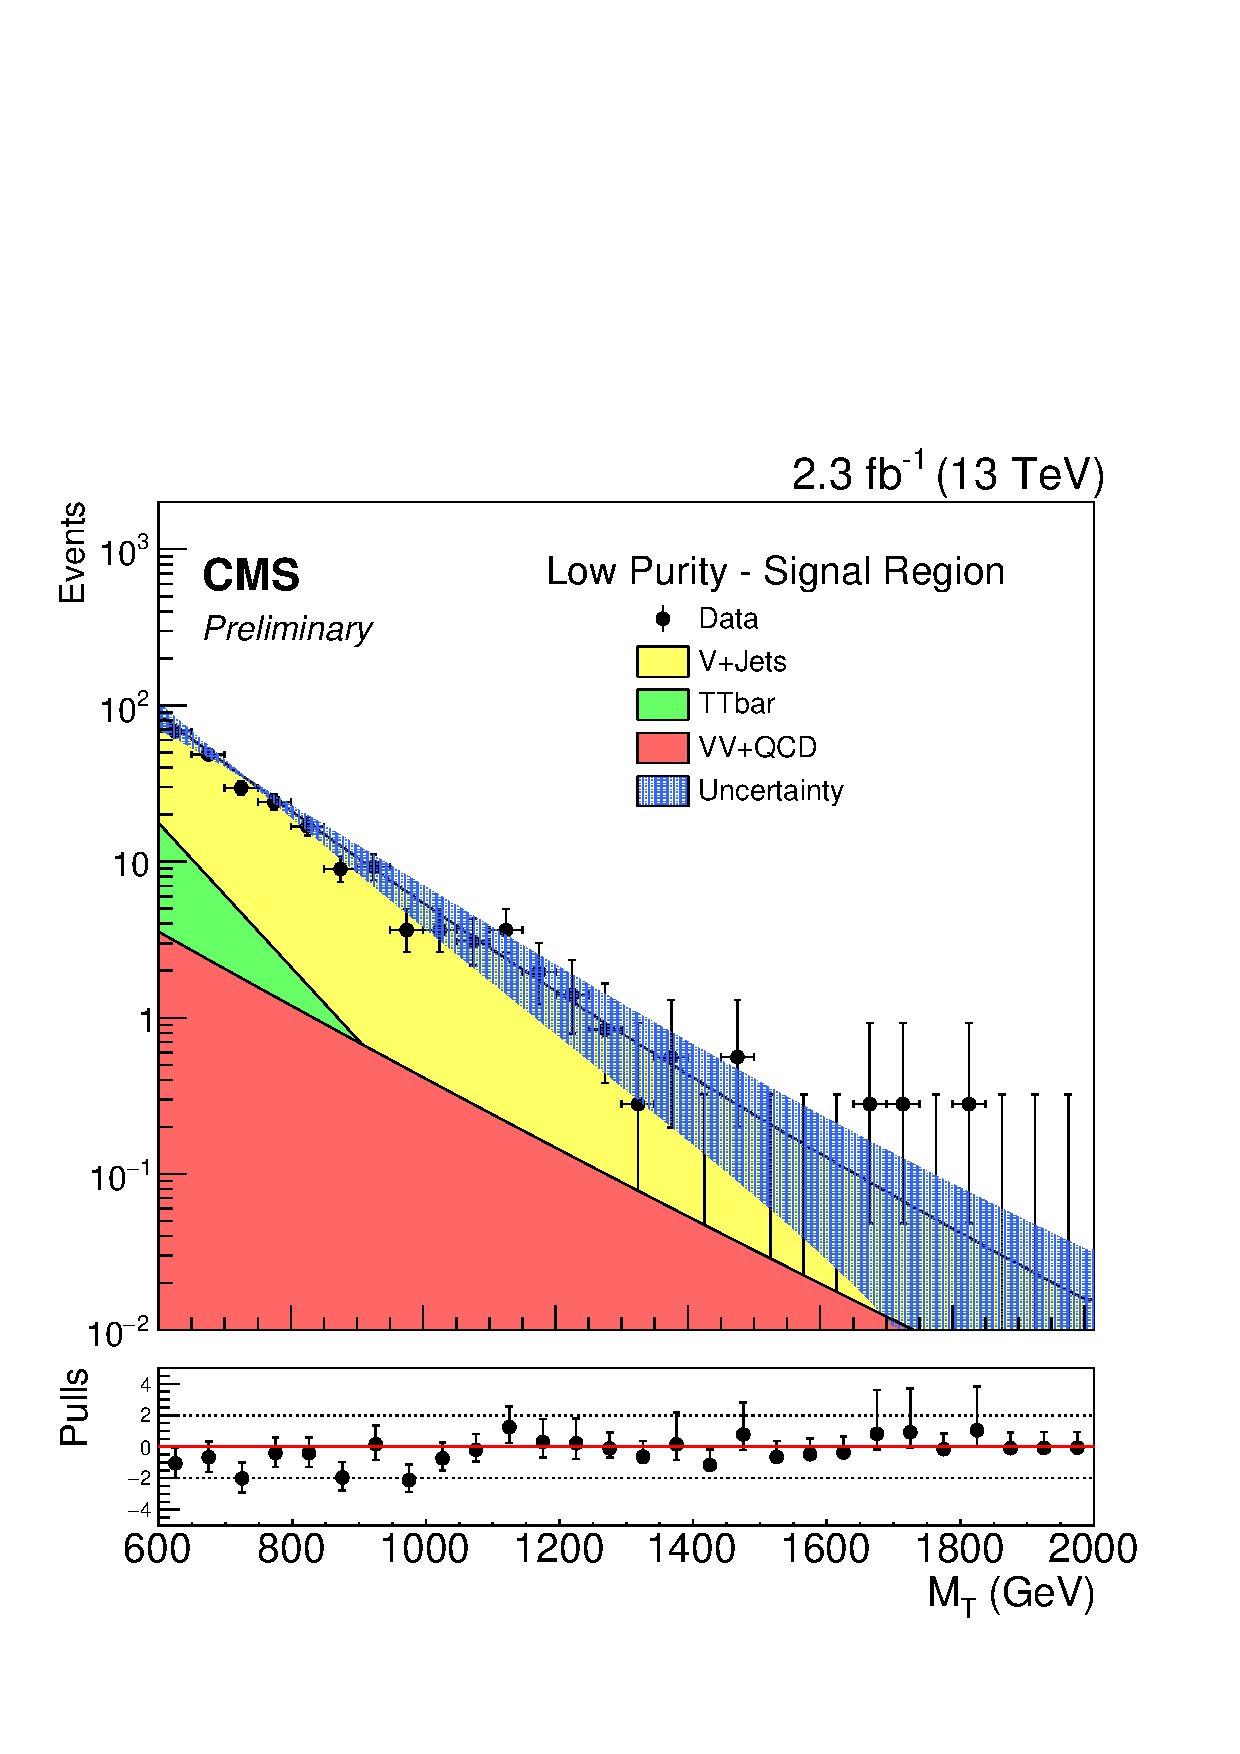
\includegraphics[width=200pt]{figuresARC/fits/finalresultUBLP.pdf}
\end{center}
\label{fig:fits4}
\end{figure}

